\documentclass{article}
\usepackage{iclr2027_conference}
\usepackage{graphicx}
\usepackage{booktabs}
\usepackage{amsmath}
\usepackage{amssymb}
\usepackage{multirow}
\usepackage{xcolor}
\usepackage{tikz}
\usetikzlibrary{positioning,calc}
\usepackage{hyperref}
\usepackage{url}
%%%%% NEW MATH DEFINITIONS %%%%%

\usepackage{amsmath,amsfonts,bm}

% Mark sections of captions for referring to divisions of figures
\newcommand{\figleft}{{\em (Left)}}
\newcommand{\figcenter}{{\em (Center)}}
\newcommand{\figright}{{\em (Right)}}
\newcommand{\figtop}{{\em (Top)}}
\newcommand{\figbottom}{{\em (Bottom)}}
\newcommand{\captiona}{{\em (a)}}
\newcommand{\captionb}{{\em (b)}}
\newcommand{\captionc}{{\em (c)}}
\newcommand{\captiond}{{\em (d)}}

% Highlight a newly defined term
\newcommand{\newterm}[1]{{\bf #1}}


% Figure reference, lower-case.
\def\figref#1{figure~\ref{#1}}
% Figure reference, capital. For start of sentence
\def\Figref#1{Figure~\ref{#1}}
\def\twofigref#1#2{figures \ref{#1} and \ref{#2}}
\def\quadfigref#1#2#3#4{figures \ref{#1}, \ref{#2}, \ref{#3} and \ref{#4}}
% Section reference, lower-case.
\def\secref#1{section~\ref{#1}}
% Section reference, capital.
\def\Secref#1{Section~\ref{#1}}
% Reference to two sections.
\def\twosecrefs#1#2{sections \ref{#1} and \ref{#2}}
% Reference to three sections.
\def\secrefs#1#2#3{sections \ref{#1}, \ref{#2} and \ref{#3}}
% Reference to an equation, lower-case.
\def\eqref#1{equation~\ref{#1}}
% Reference to an equation, upper case
\def\Eqref#1{Equation~\ref{#1}}
% A raw reference to an equation---avoid using if possible
\def\plaineqref#1{\ref{#1}}
% Reference to a chapter, lower-case.
\def\chapref#1{chapter~\ref{#1}}
% Reference to an equation, upper case.
\def\Chapref#1{Chapter~\ref{#1}}
% Reference to a range of chapters
\def\rangechapref#1#2{chapters\ref{#1}--\ref{#2}}
% Reference to an algorithm, lower-case.
\def\algref#1{algorithm~\ref{#1}}
% Reference to an algorithm, upper case.
\def\Algref#1{Algorithm~\ref{#1}}
\def\twoalgref#1#2{algorithms \ref{#1} and \ref{#2}}
\def\Twoalgref#1#2{Algorithms \ref{#1} and \ref{#2}}
% Reference to a part, lower case
\def\partref#1{part~\ref{#1}}
% Reference to a part, upper case
\def\Partref#1{Part~\ref{#1}}
\def\twopartref#1#2{parts \ref{#1} and \ref{#2}}

\def\ceil#1{\lceil #1 \rceil}
\def\floor#1{\lfloor #1 \rfloor}
\def\1{\bm{1}}
\newcommand{\train}{\mathcal{D}}
\newcommand{\valid}{\mathcal{D_{\mathrm{valid}}}}
\newcommand{\test}{\mathcal{D_{\mathrm{test}}}}

\def\eps{{\epsilon}}


% Random variables
\def\reta{{\textnormal{$\eta$}}}
\def\ra{{\textnormal{a}}}
\def\rb{{\textnormal{b}}}
\def\rc{{\textnormal{c}}}
\def\rd{{\textnormal{d}}}
\def\re{{\textnormal{e}}}
\def\rf{{\textnormal{f}}}
\def\rg{{\textnormal{g}}}
\def\rh{{\textnormal{h}}}
\def\ri{{\textnormal{i}}}
\def\rj{{\textnormal{j}}}
\def\rk{{\textnormal{k}}}
\def\rl{{\textnormal{l}}}
% rm is already a command, just don't name any random variables m
\def\rn{{\textnormal{n}}}
\def\ro{{\textnormal{o}}}
\def\rp{{\textnormal{p}}}
\def\rq{{\textnormal{q}}}
\def\rr{{\textnormal{r}}}
\def\rs{{\textnormal{s}}}
\def\rt{{\textnormal{t}}}
\def\ru{{\textnormal{u}}}
\def\rv{{\textnormal{v}}}
\def\rw{{\textnormal{w}}}
\def\rx{{\textnormal{x}}}
\def\ry{{\textnormal{y}}}
\def\rz{{\textnormal{z}}}

% Random vectors
\def\rvepsilon{{\mathbf{\epsilon}}}
\def\rvtheta{{\mathbf{\theta}}}
\def\rva{{\mathbf{a}}}
\def\rvb{{\mathbf{b}}}
\def\rvc{{\mathbf{c}}}
\def\rvd{{\mathbf{d}}}
\def\rve{{\mathbf{e}}}
\def\rvf{{\mathbf{f}}}
\def\rvg{{\mathbf{g}}}
\def\rvh{{\mathbf{h}}}
\def\rvu{{\mathbf{i}}}
\def\rvj{{\mathbf{j}}}
\def\rvk{{\mathbf{k}}}
\def\rvl{{\mathbf{l}}}
\def\rvm{{\mathbf{m}}}
\def\rvn{{\mathbf{n}}}
\def\rvo{{\mathbf{o}}}
\def\rvp{{\mathbf{p}}}
\def\rvq{{\mathbf{q}}}
\def\rvr{{\mathbf{r}}}
\def\rvs{{\mathbf{s}}}
\def\rvt{{\mathbf{t}}}
\def\rvu{{\mathbf{u}}}
\def\rvv{{\mathbf{v}}}
\def\rvw{{\mathbf{w}}}
\def\rvx{{\mathbf{x}}}
\def\rvy{{\mathbf{y}}}
\def\rvz{{\mathbf{z}}}

% Elements of random vectors
\def\erva{{\textnormal{a}}}
\def\ervb{{\textnormal{b}}}
\def\ervc{{\textnormal{c}}}
\def\ervd{{\textnormal{d}}}
\def\erve{{\textnormal{e}}}
\def\ervf{{\textnormal{f}}}
\def\ervg{{\textnormal{g}}}
\def\ervh{{\textnormal{h}}}
\def\ervi{{\textnormal{i}}}
\def\ervj{{\textnormal{j}}}
\def\ervk{{\textnormal{k}}}
\def\ervl{{\textnormal{l}}}
\def\ervm{{\textnormal{m}}}
\def\ervn{{\textnormal{n}}}
\def\ervo{{\textnormal{o}}}
\def\ervp{{\textnormal{p}}}
\def\ervq{{\textnormal{q}}}
\def\ervr{{\textnormal{r}}}
\def\ervs{{\textnormal{s}}}
\def\ervt{{\textnormal{t}}}
\def\ervu{{\textnormal{u}}}
\def\ervv{{\textnormal{v}}}
\def\ervw{{\textnormal{w}}}
\def\ervx{{\textnormal{x}}}
\def\ervy{{\textnormal{y}}}
\def\ervz{{\textnormal{z}}}

% Random matrices
\def\rmA{{\mathbf{A}}}
\def\rmB{{\mathbf{B}}}
\def\rmC{{\mathbf{C}}}
\def\rmD{{\mathbf{D}}}
\def\rmE{{\mathbf{E}}}
\def\rmF{{\mathbf{F}}}
\def\rmG{{\mathbf{G}}}
\def\rmH{{\mathbf{H}}}
\def\rmI{{\mathbf{I}}}
\def\rmJ{{\mathbf{J}}}
\def\rmK{{\mathbf{K}}}
\def\rmL{{\mathbf{L}}}
\def\rmM{{\mathbf{M}}}
\def\rmN{{\mathbf{N}}}
\def\rmO{{\mathbf{O}}}
\def\rmP{{\mathbf{P}}}
\def\rmQ{{\mathbf{Q}}}
\def\rmR{{\mathbf{R}}}
\def\rmS{{\mathbf{S}}}
\def\rmT{{\mathbf{T}}}
\def\rmU{{\mathbf{U}}}
\def\rmV{{\mathbf{V}}}
\def\rmW{{\mathbf{W}}}
\def\rmX{{\mathbf{X}}}
\def\rmY{{\mathbf{Y}}}
\def\rmZ{{\mathbf{Z}}}

% Elements of random matrices
\def\ermA{{\textnormal{A}}}
\def\ermB{{\textnormal{B}}}
\def\ermC{{\textnormal{C}}}
\def\ermD{{\textnormal{D}}}
\def\ermE{{\textnormal{E}}}
\def\ermF{{\textnormal{F}}}
\def\ermG{{\textnormal{G}}}
\def\ermH{{\textnormal{H}}}
\def\ermI{{\textnormal{I}}}
\def\ermJ{{\textnormal{J}}}
\def\ermK{{\textnormal{K}}}
\def\ermL{{\textnormal{L}}}
\def\ermM{{\textnormal{M}}}
\def\ermN{{\textnormal{N}}}
\def\ermO{{\textnormal{O}}}
\def\ermP{{\textnormal{P}}}
\def\ermQ{{\textnormal{Q}}}
\def\ermR{{\textnormal{R}}}
\def\ermS{{\textnormal{S}}}
\def\ermT{{\textnormal{T}}}
\def\ermU{{\textnormal{U}}}
\def\ermV{{\textnormal{V}}}
\def\ermW{{\textnormal{W}}}
\def\ermX{{\textnormal{X}}}
\def\ermY{{\textnormal{Y}}}
\def\ermZ{{\textnormal{Z}}}

% Vectors
\def\vzero{{\bm{0}}}
\def\vone{{\bm{1}}}
\def\vmu{{\bm{\mu}}}
\def\vtheta{{\bm{\theta}}}
\def\va{{\bm{a}}}
\def\vb{{\bm{b}}}
\def\vc{{\bm{c}}}
\def\vd{{\bm{d}}}
\def\ve{{\bm{e}}}
\def\vf{{\bm{f}}}
\def\vg{{\bm{g}}}
\def\vh{{\bm{h}}}
\def\vi{{\bm{i}}}
\def\vj{{\bm{j}}}
\def\vk{{\bm{k}}}
\def\vl{{\bm{l}}}
\def\vm{{\bm{m}}}
\def\vn{{\bm{n}}}
\def\vo{{\bm{o}}}
\def\vp{{\bm{p}}}
\def\vq{{\bm{q}}}
\def\vr{{\bm{r}}}
\def\vs{{\bm{s}}}
\def\vt{{\bm{t}}}
\def\vu{{\bm{u}}}
\def\vv{{\bm{v}}}
\def\vw{{\bm{w}}}
\def\vx{{\bm{x}}}
\def\vy{{\bm{y}}}
\def\vz{{\bm{z}}}

% Elements of vectors
\def\evalpha{{\alpha}}
\def\evbeta{{\beta}}
\def\evepsilon{{\epsilon}}
\def\evlambda{{\lambda}}
\def\evomega{{\omega}}
\def\evmu{{\mu}}
\def\evpsi{{\psi}}
\def\evsigma{{\sigma}}
\def\evtheta{{\theta}}
\def\eva{{a}}
\def\evb{{b}}
\def\evc{{c}}
\def\evd{{d}}
\def\eve{{e}}
\def\evf{{f}}
\def\evg{{g}}
\def\evh{{h}}
\def\evi{{i}}
\def\evj{{j}}
\def\evk{{k}}
\def\evl{{l}}
\def\evm{{m}}
\def\evn{{n}}
\def\evo{{o}}
\def\evp{{p}}
\def\evq{{q}}
\def\evr{{r}}
\def\evs{{s}}
\def\evt{{t}}
\def\evu{{u}}
\def\evv{{v}}
\def\evw{{w}}
\def\evx{{x}}
\def\evy{{y}}
\def\evz{{z}}

% Matrix
\def\mA{{\bm{A}}}
\def\mB{{\bm{B}}}
\def\mC{{\bm{C}}}
\def\mD{{\bm{D}}}
\def\mE{{\bm{E}}}
\def\mF{{\bm{F}}}
\def\mG{{\bm{G}}}
\def\mH{{\bm{H}}}
\def\mI{{\bm{I}}}
\def\mJ{{\bm{J}}}
\def\mK{{\bm{K}}}
\def\mL{{\bm{L}}}
\def\mM{{\bm{M}}}
\def\mN{{\bm{N}}}
\def\mO{{\bm{O}}}
\def\mP{{\bm{P}}}
\def\mQ{{\bm{Q}}}
\def\mR{{\bm{R}}}
\def\mS{{\bm{S}}}
\def\mT{{\bm{T}}}
\def\mU{{\bm{U}}}
\def\mV{{\bm{V}}}
\def\mW{{\bm{W}}}
\def\mX{{\bm{X}}}
\def\mY{{\bm{Y}}}
\def\mZ{{\bm{Z}}}
\def\mBeta{{\bm{\beta}}}
\def\mPhi{{\bm{\Phi}}}
\def\mLambda{{\bm{\Lambda}}}
\def\mSigma{{\bm{\Sigma}}}

% Tensor
\DeclareMathAlphabet{\mathsfit}{\encodingdefault}{\sfdefault}{m}{sl}
\SetMathAlphabet{\mathsfit}{bold}{\encodingdefault}{\sfdefault}{bx}{n}
\newcommand{\tens}[1]{\bm{\mathsfit{#1}}}
\def\tA{{\tens{A}}}
\def\tB{{\tens{B}}}
\def\tC{{\tens{C}}}
\def\tD{{\tens{D}}}
\def\tE{{\tens{E}}}
\def\tF{{\tens{F}}}
\def\tG{{\tens{G}}}
\def\tH{{\tens{H}}}
\def\tI{{\tens{I}}}
\def\tJ{{\tens{J}}}
\def\tK{{\tens{K}}}
\def\tL{{\tens{L}}}
\def\tM{{\tens{M}}}
\def\tN{{\tens{N}}}
\def\tO{{\tens{O}}}
\def\tP{{\tens{P}}}
\def\tQ{{\tens{Q}}}
\def\tR{{\tens{R}}}
\def\tS{{\tens{S}}}
\def\tT{{\tens{T}}}
\def\tU{{\tens{U}}}
\def\tV{{\tens{V}}}
\def\tW{{\tens{W}}}
\def\tX{{\tens{X}}}
\def\tY{{\tens{Y}}}
\def\tZ{{\tens{Z}}}


% Graph
\def\gA{{\mathcal{A}}}
\def\gB{{\mathcal{B}}}
\def\gC{{\mathcal{C}}}
\def\gD{{\mathcal{D}}}
\def\gE{{\mathcal{E}}}
\def\gF{{\mathcal{F}}}
\def\gG{{\mathcal{G}}}
\def\gH{{\mathcal{H}}}
\def\gI{{\mathcal{I}}}
\def\gJ{{\mathcal{J}}}
\def\gK{{\mathcal{K}}}
\def\gL{{\mathcal{L}}}
\def\gM{{\mathcal{M}}}
\def\gN{{\mathcal{N}}}
\def\gO{{\mathcal{O}}}
\def\gP{{\mathcal{P}}}
\def\gQ{{\mathcal{Q}}}
\def\gR{{\mathcal{R}}}
\def\gS{{\mathcal{S}}}
\def\gT{{\mathcal{T}}}
\def\gU{{\mathcal{U}}}
\def\gV{{\mathcal{V}}}
\def\gW{{\mathcal{W}}}
\def\gX{{\mathcal{X}}}
\def\gY{{\mathcal{Y}}}
\def\gZ{{\mathcal{Z}}}

% Sets
\def\sA{{\mathbb{A}}}
\def\sB{{\mathbb{B}}}
\def\sC{{\mathbb{C}}}
\def\sD{{\mathbb{D}}}
% Don't use a set called E, because this would be the same as our symbol
% for expectation.
\def\sF{{\mathbb{F}}}
\def\sG{{\mathbb{G}}}
\def\sH{{\mathbb{H}}}
\def\sI{{\mathbb{I}}}
\def\sJ{{\mathbb{J}}}
\def\sK{{\mathbb{K}}}
\def\sL{{\mathbb{L}}}
\def\sM{{\mathbb{M}}}
\def\sN{{\mathbb{N}}}
\def\sO{{\mathbb{O}}}
\def\sP{{\mathbb{P}}}
\def\sQ{{\mathbb{Q}}}
\def\sR{{\mathbb{R}}}
\def\sS{{\mathbb{S}}}
\def\sT{{\mathbb{T}}}
\def\sU{{\mathbb{U}}}
\def\sV{{\mathbb{V}}}
\def\sW{{\mathbb{W}}}
\def\sX{{\mathbb{X}}}
\def\sY{{\mathbb{Y}}}
\def\sZ{{\mathbb{Z}}}

% Entries of a matrix
\def\emLambda{{\Lambda}}
\def\emA{{A}}
\def\emB{{B}}
\def\emC{{C}}
\def\emD{{D}}
\def\emE{{E}}
\def\emF{{F}}
\def\emG{{G}}
\def\emH{{H}}
\def\emI{{I}}
\def\emJ{{J}}
\def\emK{{K}}
\def\emL{{L}}
\def\emM{{M}}
\def\emN{{N}}
\def\emO{{O}}
\def\emP{{P}}
\def\emQ{{Q}}
\def\emR{{R}}
\def\emS{{S}}
\def\emT{{T}}
\def\emU{{U}}
\def\emV{{V}}
\def\emW{{W}}
\def\emX{{X}}
\def\emY{{Y}}
\def\emZ{{Z}}
\def\emSigma{{\Sigma}}

% entries of a tensor
% Same font as tensor, without \bm wrapper
\newcommand{\etens}[1]{\mathsfit{#1}}
\def\etLambda{{\etens{\Lambda}}}
\def\etA{{\etens{A}}}
\def\etB{{\etens{B}}}
\def\etC{{\etens{C}}}
\def\etD{{\etens{D}}}
\def\etE{{\etens{E}}}
\def\etF{{\etens{F}}}
\def\etG{{\etens{G}}}
\def\etH{{\etens{H}}}
\def\etI{{\etens{I}}}
\def\etJ{{\etens{J}}}
\def\etK{{\etens{K}}}
\def\etL{{\etens{L}}}
\def\etM{{\etens{M}}}
\def\etN{{\etens{N}}}
\def\etO{{\etens{O}}}
\def\etP{{\etens{P}}}
\def\etQ{{\etens{Q}}}
\def\etR{{\etens{R}}}
\def\etS{{\etens{S}}}
\def\etT{{\etens{T}}}
\def\etU{{\etens{U}}}
\def\etV{{\etens{V}}}
\def\etW{{\etens{W}}}
\def\etX{{\etens{X}}}
\def\etY{{\etens{Y}}}
\def\etZ{{\etens{Z}}}

% The true underlying data generating distribution
\newcommand{\pdata}{p_{\rm{data}}}
% The empirical distribution defined by the training set
\newcommand{\ptrain}{\hat{p}_{\rm{data}}}
\newcommand{\Ptrain}{\hat{P}_{\rm{data}}}
% The model distribution
\newcommand{\pmodel}{p_{\rm{model}}}
\newcommand{\Pmodel}{P_{\rm{model}}}
\newcommand{\ptildemodel}{\tilde{p}_{\rm{model}}}
% Stochastic autoencoder distributions
\newcommand{\pencode}{p_{\rm{encoder}}}
\newcommand{\pdecode}{p_{\rm{decoder}}}
\newcommand{\precons}{p_{\rm{reconstruct}}}

\newcommand{\laplace}{\mathrm{Laplace}} % Laplace distribution

\newcommand{\E}{\mathbb{E}}
\newcommand{\Ls}{\mathcal{L}}
\newcommand{\R}{\mathbb{R}}
\newcommand{\emp}{\tilde{p}}
\newcommand{\lr}{\alpha}
\newcommand{\reg}{\lambda}
\newcommand{\rect}{\mathrm{rectifier}}
\newcommand{\softmax}{\mathrm{softmax}}
\newcommand{\sigmoid}{\sigma}
\newcommand{\softplus}{\zeta}
\newcommand{\KL}{D_{\mathrm{KL}}}
\newcommand{\Var}{\mathrm{Var}}
\newcommand{\standarderror}{\mathrm{SE}}
\newcommand{\Cov}{\mathrm{Cov}}
% Wolfram Mathworld says $L^2$ is for function spaces and $\ell^2$ is for vectors
% But then they seem to use $L^2$ for vectors throughout the site, and so does
% wikipedia.
\newcommand{\normlzero}{L^0}
\newcommand{\normlone}{L^1}
\newcommand{\normltwo}{L^2}
\newcommand{\normlp}{L^p}
\newcommand{\normmax}{L^\infty}

\newcommand{\parents}{Pa} % See usage in notation.tex. Chosen to match Daphne's book.

\DeclareMathOperator*{\argmax}{arg\,max}
\DeclareMathOperator*{\argmin}{arg\,min}

\DeclareMathOperator{\sign}{sign}
\DeclareMathOperator{\Tr}{Tr}
\let\ab\allowbreak


\newcommand{\TBD}[1]{\textcolor{red}{\textbf{[TBD: #1]}}}
\newcommand{\EHS}{\mathrm{EHS}}

\title{How Far Back Should We Look? Measuring, Explaining, and Exploiting\\ the Effective History Span of Time Series Forecasting}

\author{Anonymous Authors}

\begin{document}
\maketitle

\begin{abstract}
Every time series forecasting model consumes a fixed-length history window, yet the window length is chosen by convention rather than by evidence. We show that this convention is silently expensive. Under a protocol that holds the training data budget fixed, the optimal lookback varies by 30x across benchmarks: exchange-rate forecasting is best at 96 steps and degrades 3.6x with longer inputs, while electricity and traffic keep improving up to 2880 steps. The pattern replicates without any training in a zero-shot foundation model, so it is a property of the data--model pairing, not of a training procedure. We explain the divergence with a two-axis account: distant history benefits through periodic and long-memory structure that survives regime changes, and harms through non-stationary drift that turns old windows into contaminated samples. The natural single-axis alternative---the span equals the expected run length of a changepoint model---is falsified: the most regime-switching datasets have the longest optimal lookbacks. The effective span is partially predictable from cheap, training-free statistics of the training data alone (leave-one-dataset-out Spearman $|\rho| = 0.63$ over fourteen public datasets), and the failure of standard architectures to suppress stale content is mechanical: attention flattens with context length, and even a linear model does not learn to gate out distant lags. On controlled synthetic series the harm axis obeys an empirical law, $W^* \propto \lambda^{-1/3}$ in the drift rate $\lambda$, which refutes the classical $-2/3$ exponent of continuous-drift estimation and prescribes a drift-matched exponential input decay; on real benchmarks the calibrated decay saturates to a universal safe default that never degrades the no-budget baseline. A hard input budget recovers 74--98\% of the long-context degradation on trained patch-family models, and budgeted truncation of a frozen foundation model matches validation-based span selection on all eight benchmarks tested. Our results argue that lookback should be treated as a measurable, predictable, data-dependent resource rather than a convention.
\end{abstract}



\begin{figure*}[t]
  \centering
  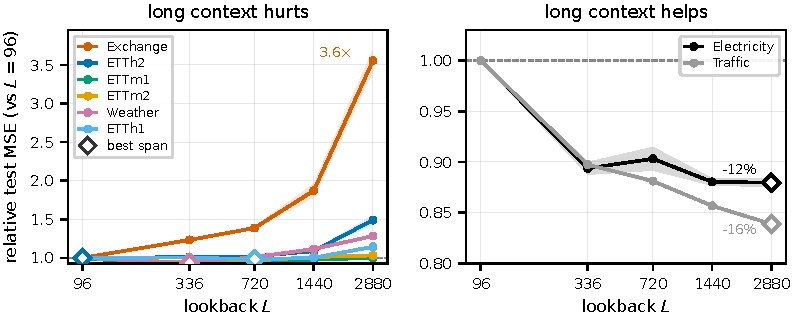
\includegraphics[width=0.55\textwidth]{figs/fig1_sweep.pdf}
  \caption{Relative test MSE (each dataset normalized to its own $L{=}96$) versus lookback under the equal-data-budget protocol (iTransformer, three seeds, mean $\pm$ std). Same model, same training data budget; only the input length changes. Left: datasets where long context hurts (drift-dominated). Right: datasets where long context helps (periodicity-dominated). Diamonds mark each dataset's best span $L^*$ (argmin over the lookback grid; the parsimonious EHS variant is analyzed in Appendix \ref{app:robust}). Cells with partial seed coverage are noted in Appendix \ref{app:ledger}.}
  \label{fig:sweep}
\end{figure*}

\section{Introduction}

Time series forecasting models map a history window of length $L$ to a future horizon. The choice of $L$ is one of the oldest decisions in the field, and one of the least examined. Classical practice selects it by autocorrelation diagnostics; the deep learning era replaced diagnostics with convention: the widely used long-term forecasting benchmark suite fixes $L = 96$ or $336$ for nearly every model and dataset \citep{dlinear, patchtst, itransformer, timesnet}, and extensions past a few hundred steps rarely help \citep{dlinear}. Foundation models pushed the window to thousands of steps \citep{chronos, timesfm, toto2}, and inference-time schemes stretch it further by downsampling \citep{sprint}. Across both eras, the implicit assumption is that history is a resource: more of it should not hurt, and probably helps.

We find that this assumption is wrong in a measurable, predictable, and exploitable way. Figure \ref{fig:sweep} shows the basic phenomenon. Holding the number of training windows exactly constant across lookback lengths, the test error of a standard forecaster traces a U-shape whose minimum moves by a factor of 30 across datasets: 96 steps on exchange rates, 336 on weather and minute-level ETT, 720 on ETTh1, and still improving at 2880 on electricity and traffic. The same ordering at the two poles (shortest on exchange, longest on traffic and electricity) appears in a zero-shot foundation model whose training never saw the decisive benchmark: traffic is confirmed absent from its pretraining corpus, and the one corpus overlap we find, electricity, is disclosed in Section \ref{sec:zero}. This rules out explanations based on optimization dynamics or overfitting to a training split. Lookback behaves like a resource with a dataset-specific point of diminishing, then negative, returns. We call this point the \emph{effective history span} (EHS) of a forecasting problem.

Why should distant history ever hurt? The information-theoretic intuition that more context cannot reduce a sufficient model's performance fails on time series for a structural reason: the data-generating process drifts. Windows drawn from an old regime carry an outdated conditional mapping, and empirical risk minimization mixes the old mapping with the new one. The pollution account, however, is only half of the story. We show that a single-axis theory, in which the useful history is the time since the last regime change, makes a sharp prediction---that regime-switching data should demand short windows---which is cleanly falsified: electricity and traffic switch regimes most frequently among our benchmarks, yet benefit from the longest lookbacks (Section \ref{sec:bocpd}). The resolution is a two-axis account. Non-stationarity sets the cost of distant history; periodic and long-memory structure sets its benefit, because such structure is invariant across regimes. Electricity's weekly cycle survives every regime change, while the level of a drifting exchange rate does not. The effective history span is the balance of the two axes.

This account has four consequences that we develop into results. First, the harm axis obeys a quantitative law: on controlled synthetic drift the best span scales as $W^* \propto \lambda^{-1/3}$ in the drift rate $\lambda$, refuting the classical $-2/3$ exponent (Section \ref{sec:powerlaw}). Second, the inability of standard architectures to exploit long context is mechanical and inspectable: attention weights flatten with context, no sink forms to absorb stale mass, linear models do not learn to zero distant lags, and the projection head keeps reading the full window under masking (Section \ref{sec:mechanism}). Third, the EHS is partially predictable before any training: simple context statistics, a segment-mean drift index and long-lag autocorrelation, achieve Spearman $|\rho| = 0.83$--$0.94$ with the measured long-context benefit in a six-dataset pilot (Sections \ref{sec:predict} and \ref{sec:predictfull}). Fourth, if the diagnosis is right, then allocating history like a budget should recover the loss: an input budget recovers 74--98\% of the degradation on trained patch-family models, and a statistics-guided budget on a frozen foundation model matches validation-based span selection on all eight benchmarks tested (Sections \ref{sec:predictfull} and \ref{sec:method}).

\paragraph{Contributions.}
\begin{itemize}
    \item We define the effective history span and provide a confound-controlled measurement protocol that separates window length from training data quantity (Section \ref{sec:measure}).
    \item We establish the two-axis account of when distant history helps or hurts, falsifying the single-axis changepoint alternative (Section \ref{sec:why}).
    \item We show that the EHS is partially predictable from cheap, leakage-free context statistics---the only zero-cost selector that identifies long-span datasets, where PACF/AIC order selection fail structurally---and, for a frozen foundation model, a statistic rule matches validation-based span selection at zero cost (Section \ref{sec:predictfull}).
    \item We diagnose why architectures fail to exploit long context, measure a power law $W^* \propto \lambda^{-1/3}$ for the harm axis, and introduce history budgeting, an input-side module allocating history per window (Sections \ref{sec:mechanism}--\ref{sec:method}).
\end{itemize}

\section{Related Work}
\label{sec:related}

\paragraph{Lookback length in deep forecasting.}
The long-term forecasting benchmark suite standardized $L \in \{96, 336\}$ following the protocol of \citet{informer} and \citet{autoformer}. \citet{dlinear} showed linear models match or beat transformers at these lengths and reported flat returns past a few hundred steps; later work kept the convention \citep{patchtst, timesnet, itransformer, timemixer}. Periodic structure has been modeled explicitly \citep{cyclenet, koopa}, instance normalization addresses level shift between windows \citep{revin}, and frequency-domain normalization removes non-stationary components instance-wise \citep{fan}. Retrieval over similar past windows outperforms long contexts on stochastic series, with an inverse scaling law for patch transformers \citep{raft, inversescaling}, and multi-scale decompositions of long context beat naive downsampling \citep{contextbottleneck}. None of these works measure how much history is usable; retrieval selects \emph{which} distant windows to read, while we ask how much of the distant window's \emph{content} survives drift. The closest neighbors are \citet{tamer}, who study the importance distribution \emph{within} a fixed window of 96 steps, and \citet{sprint}, who extend context at inference time by downsampling under an implicit longer-is-better assumption; our exchange-rate results are a direct counterexample to that assumption. On the horizon side, \citet{fern} propose effective prediction time, a measure of how far forward a forecast remains reliable; our EHS is the input-side dual. In language modeling, \citet{lostinthemiddle} measure how poorly models use the middle of long contexts, a sibling phenomenon with a different cause.

\paragraph{Foundation models and scaling.}
Zero-shot forecasters \citep{chronos, timesfm} and billion-scale models \citep{toto2} moved the field toward large pretraining corpora and larger contexts, tracked by recent benchmarks \citep{gifteval, timebench}. Routing across a pool of foundation models \citep{timerouter} and correlation-aware adaptation \citep{cora} treat the model, not the history, as the object to be selected. A separate engineering line treats lookback as a hyperparameter to tune per dataset \citep{timemixer, letsforecast}; tuning answers \emph{which} span wins on a validation split, while we ask \emph{why} a span wins, whether the answer can be computed without training, and what breaks when the span is wrong. Analyses of positional encoding find that positional topology degrades with depth \citep{tem, pesurvey}; our attention-entropy measurements extend this line from encodings to the usage of distant content itself.

\paragraph{Non-stationarity and regime structure.}
Distribution shift in forecasting is classically handled by reversible normalization \citep{revin} and by models of switching dynamics, from Markov-switching econometrics to Bayesian online changepoint detection \citep{bocpd} and deep switching state-space models. The statistical literature selects the estimation window itself under drift, through forgetting-factor recursive identification \citep{ljung1983} and adaptive window selection for risk forecasting \citep{adaptivewindow}; these methods window a classical estimator, while we measure, predict, and budget the usable span of deep forecasters and foundation models. We use the changepoint formalism as a hypothesis to test rather than as an assumption (Section \ref{sec:bocpd}).

\section{Measuring the Effective History Span}
\label{sec:measure}

\paragraph{Setup.}
We consider multivariate forecasting with a history window $x_{t-L+1:t}$ and a horizon of $H=96$ steps, following the standard protocol \citep{dlinear, itransformer}. A lookback sweep varies $L \in \{96, 336, 720, 1440, 2880\}$. The confound we remove first is that longer windows reduce the number of available training windows, so any degradation could be attributed to data quantity rather than window content. Our protocol holds the number of training windows exactly constant at the count available under the longest lookback, subsampling uniformly for all shorter lookbacks (Appendix \ref{app:protocol}). We sweep four model families that differ in how history enters the computation, iTransformer \citep{itransformer} (attention across variates), PatchTST \citep{patchtst} (attention across patches), TimesNet \citep{timesnet} (2D convolutions over folded periods), and DLinear \citep{dlinear} (per-channel linear maps), on eight benchmarks (ETTh1, ETTh2, ETTm1, ETTm2, exchange rate, weather, electricity, traffic), three seeds each (the complete run ledger, including initially failed arms and their re-runs, is documented in Appendix \ref{app:ledger}).

\begin{table}[t]
\caption{Test MSE under the equal-data-budget protocol (iTransformer, three seeds per cell; full matrix in Appendix \ref{app:full}). Bold marks the best lookback within each row. The optimal lookback varies 30x across datasets.}
\label{tab:main}
\centering\scriptsize
\begin{tabular}{lcccccc}
\toprule
Dataset & $L{=}96$ & $L{=}336$ & $L{=}720$ & $L{=}1440$ & $L{=}2880$ & Best \\
\midrule
ETTh1 & 0.399 & 0.402 & \textbf{0.392} & 0.400 & 0.457 & 720 \\
ETTh2 & \textbf{0.299} & 0.302 & 0.305 & 0.325 & 0.445 & 96 \\
ETTm1 & 0.342 & \textbf{0.304} & 0.313 & 0.336 & 0.341 & 336 \\
ETTm2 & 0.185 & \textbf{0.174} & 0.179 & 0.187 & 0.191 & 336 \\
Electricity & 0.149 & 0.133 & 0.134 & 0.131 & \textbf{0.131} & 2880 \\
Exchange & \textbf{0.089} & 0.110 & 0.123 & 0.166 & 0.316 & 96 \\
Traffic & 0.406 & 0.365 & 0.358 & 0.348 & \textbf{0.341} & 2880 \\
Weather & 0.175 & \textbf{0.163} & 0.177 & 0.195 & 0.225 & 336 \\
\bottomrule
\end{tabular}
\end{table}


\paragraph{The divergence is real and large.}
Table \ref{tab:main} shows the controlled sweep for iTransformer. With the data budget held fixed, exchange rate degrades monotonically from 0.089 at $L{=}96$ to 0.316 at $L{=}2880$ (3.6x), while traffic improves monotonically from 0.406 to 0.341 ($-$16\%). Seed noise is far smaller than the lookback effect: the median per-seed standard deviation is 1.0\% of the cell mean across the full 480-run matrix, and the largest deviations occur in already-degraded long-window cells, where they change no ranking (the full distribution is in Appendix \ref{app:full}). Extending the sweep to $L{=}5760$ on electricity and traffic confirms that the benefit plateaus between $L{=}1440$ and $L{=}2880$ rather than being clipped by the scan range: errors at $L{=}5760$ never improve over $L{=}2880$ (Appendix \ref{app:full}). Table \ref{tab:bestl} summarizes the best lookback per model family: the data-side ordering---exchange shortest, electricity and traffic longest---is consistent across iTransformer, DLinear, PatchTST, and the zero-shot foundation model Chronos-Bolt \citep{chronos} (Section \ref{sec:zero}). TimesNet is the exception that exposes the model-side gate: its convolutional mixing cannot exploit long context, so its optimum stays at $L{=}96$ on electricity and traffic where every attention-based family goes long.

\begin{table}[t]
\caption{Best lookback per dataset and model family (equal data budget; all trained cells carry three seeds). $\uparrow$ marks monotone improvement through the longest span tested in that row; `--' marks settings not evaluated. $^{\dagger}$Wide-data zero-shot cells are evaluated with test-stride 2, Chronos-Bolt truncates contexts beyond 2048 steps, and electricity is suspected in-domain for the original Chronos corpus while traffic is confirmed never seen. The data-side ordering is model-consistent; the model side gates whether long context helps at all.}
\label{tab:bestl}
\centering\scriptsize
\begin{tabular}{lccccc}
\toprule
Dataset & iTransformer & DLinear & PatchTST & TimesNet & Chronos (zero-shot) \\
\midrule
ETTh1 & 720 & 1440 & 336 & 96 & $\uparrow$1440 \\
ETTh2 & 96 & 720 & 96 & 96 & 1440 \\
ETTm1 & 336 & 336 & 336 & 96 & $\uparrow$1440 \\
ETTm2 & 336 & 2880 & 336 & 96 & $\uparrow$1440 \\
Electricity & 2880 & 2880 & 1440 & 96 & 1440$^{\dagger}$ \\
Exchange & 96 & 96 & 96 & 96 & 96 \\
Traffic & 2880 & 2880 & $\uparrow$2880 & 96 & $\uparrow$2880$^{\dagger}$ \\
Weather & 336 & 2880 & 720 & 336 & $\uparrow$1440 \\
\bottomrule
\end{tabular}
\end{table}


\paragraph{It is not training dynamics.}
\label{sec:zero}
Chronos-Bolt, evaluated zero-shot with no training on our corpora, shows the same qualitative trend at the two poles of the ordering: on the short-span side it prefers $L{=}96$ on exchange rate; on the long-span side it improves monotonically on traffic up to the longest tested span (MSE 1.225 $\to$ 0.372, $-70\%$), and on electricity up to $L{=}1440$ ($-41\%$). On ETTh2 and weather the foundation model prefers longer spans ($L{=}1440$) than the trained families ($L{=}96$ and $L{=}336$); Appendix \ref{app:gift} attributes this gap to its strong per-instance normalization, which keeps the drift-harm channel dormant up to much higher drift than in the trained models. Bolt's context is capped at 2048 steps, so our $L{=}2880$ zero-shot runs read 2048 effective steps, and the wide-data zero-shot cells are evaluated with test-stride 2 (Appendix \ref{app:ledger}); while traffic is confirmed never seen in pretraining, electricity appears in the original Chronos corpus, so its zero-shot numbers carry a suspected-in-domain qualification and the long-span replication rests on traffic. The phenomenon is therefore a property of how the data's structure matches the inductive bias of sequence models in general, not of a specific training run. The ordering is also stable across horizons: at $H{=}192$, the short-, flat-, and long-span classes replicate exactly on exchange, ETTh1, and electricity (Appendix \ref{app:robust}). The two-axis classification further replicates on six additional public datasets (solar, PEMS04, PEMS08, ERCOT settlement prices, Melbourne pedestrian counts, and Mexico City bike demand; Appendix \ref{app:ext}): five are periodicity-dominated with long or saturating optimal spans, and the highest-drift newcomer (ERCOT) is the only one whose iTransformer optimum is short---its calendar statistic, the largest in the suite at 0.90, saturates at one week and does not pay back a longer window.

\paragraph{Definition.}
Let $e(L)$ be the test error of a fixed model class trained under the equal-data-budget protocol with lookback $L$. We define the \emph{effective history span} as
\begin{equation}
\mathrm{EHS} = \min\Big\{L : e(L) \le \min_{L'} e(L') \cdot (1 + \varepsilon)\Big\},
\label{eq:ehs}
\end{equation}
the smallest lookback whose error is within a fraction $\varepsilon$ of the best. This parsimonious form rewards shorter, cheaper windows once returns saturate. In the main text we report the argmin span $L^* = \arg\min_L e(L)$, which is the $\varepsilon \to 0$ limit and the quantity behind every ``best lookback'' figure; the parsimonious EHS($\varepsilon$) and its sensitivity to $\varepsilon$ are reported in Appendix \ref{app:robust}. The two coincide on drift-dominated datasets with a sharp optimum (exchange, ETTh2), and differ on benefit-dominated ones with a flat error curve near the optimum (electricity: $L^*{=}2880$ but EHS($0.02$)${=}336$).

\begin{figure}[t]
  \centering
  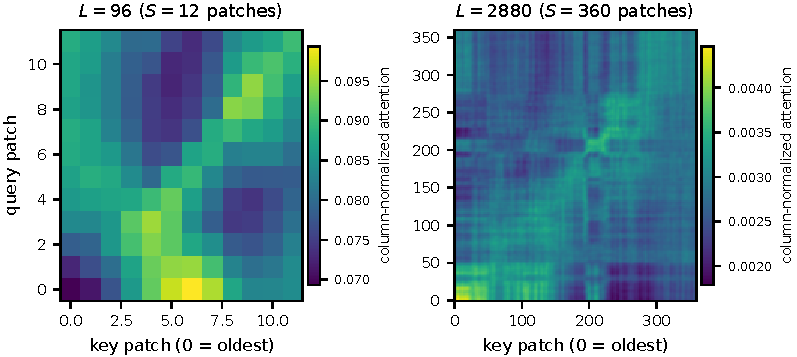
\includegraphics[width=0.60\linewidth]{figs/fig3_attention.pdf}
  \caption{Second-layer attention maps of PatchTST on exchange rate at $L{=}96$ (left) and $L{=}2880$ (right), column-normalized and averaged over heads and test batches. At long context the map flattens into broad vertical stripes (normalized entropy 0.84 $\to$ 0.91), losing discrimination without forming an attention sink.}
  \label{fig:attn}
\end{figure}

\section{What Determines the Effective History Span}
\label{sec:why}

\subsection{A single-axis theory fails}
\label{sec:bocpd}

The standard account of non-stationarity says that old data becomes useless when the regime changes. Formalizing it with Bayesian online changepoint detection \citep{bocpd} gives a sharp hypothesis: the useful history is the time since the last change, and the effective span should track the posterior expected run length $\mathbb{E}[r_t]$ of the regime process. We compute $\mathbb{E}[r_t]$ per dataset with a Gaussian unknown-mean-and-variance observation model across a hazard sweep (Appendix \ref{app:bocpd}). The hypothesis fails. The two datasets with the \emph{shortest} expected run lengths at hazard $1/50$, traffic (48 steps) and electricity (53), are precisely the ones whose optimal lookback is the \emph{longest} (2880), yielding a negative rank correlation on one model family (Spearman $\rho = -0.67$ at hazard $1/50$; we report this as pattern evidence rather than significance: the exact permutation $p$ is 0.08 and does not survive multiple-comparison control, while the negative direction persists across the hazard sweep and flips sign at the most extreme hazard). Two robustness checks close the loop (Appendix \ref{app:bocpd}): removing calendar seasonality before detection leaves the counterexample intact (phase removal keeps traffic shortest alongside the longest optimal span; seasonal differencing weakens its rank to third--fourth, still non-positive), and a changepoint-model-free drift measure independently recovers the expected negative relation ($\rho = -0.90$, Holm-adjusted $p = 0.033$ within the iTransformer statistic family). Regime persistence alone cannot explain the effective span.

\subsection{The two-axis account}

The counterexample points to the missing variable: what survives a regime change. Levels, trends, and regime parameters do not survive; periodic phase and long-memory dependence do. We therefore model the value of an old window as
\begin{equation}
V(\ell) = \underbrace{B_{\mathrm{inv}}(\ell)}_{\text{regime-invariant content}} - \underbrace{C_{\mathrm{drift}}(\ell)}_{\text{pollution cost}},
\label{eq:twoaxis}
\end{equation}
where $B_{\mathrm{inv}}$ is the information the window carries about periodic and long-memory structure (invariant across regimes), and $C_{\mathrm{drift}}$ is the cost of training on a window whose conditional mapping has expired. The EHS is the span at which the marginal benefit equals the marginal cost. This account explains the full pattern: exchange rate has high drift and weak persistent periodicity, so cost dominates at a few dozen steps; electricity and traffic switch regimes constantly but retain strong daily and weekly cycles, so distant history keeps paying; the ETT datasets sit between.

\subsection{A power law for the harm axis}
\label{sec:powerlaw}

The harm axis admits a quantitative law. A bias--variance argument predicts the optimal window under drift: bias grows with the drift accumulated over the window, variance shrinks with its length, and for continuous linear drift the predicted exponent is $W^* \propto \lambda^{-2/3}$ (derived in Appendix \ref{app:powerlaw}). We test this on controlled synthetic series whose drift rate $\lambda$ (shock probability per step) is parameterized exactly, with periodic content removed, training a small iTransformer under the equal-data-budget protocol. A first sweep over six drift tiers gives log-log slopes $-0.31$ and $-0.37$ with $R^2 = 0.82$ and $0.92$ (grid-argmin and parabolic-interpolation estimators). A hardened sweep over ten drift tiers with a refined nine-point lookback grid gives slopes $-0.29$ and $-0.32$ with $R^2 = 0.64$ and $0.76$, bootstrap intervals that contain $-\tfrac13$ and exclude $-\tfrac23$ on both estimators, and exposes a mid-drift plateau (Appendix \ref{app:powerlaw}):
\begin{equation}
W^* \propto \lambda^{-\alpha}, \qquad \alpha \approx 0.29\text{--}0.37,
\label{eq:law}
\end{equation}
because the bias of shock-driven drift scales differently from the continuous case (the shock regime sits between the naive Poisson-step prediction $-\tfrac12$ and the trend-step $-\tfrac14$). The law is family-scoped: DLinear stays short (96--480) with no monotone $\lambda$ dependence and both estimator intervals containing zero, so the power law is a coarse first description of the instance-normalized attention family, not a universal one. Two controls establish that this is the harm axis at work rather than an artifact: the drift statistic is calibrated strictly monotone in $\lambda$, and adding strong periodicity at fixed $\lambda$ extends the measured span by up to 4.3x, as the two-axis model predicts. On real benchmarks the fitted constant tracks weather (predicted 319 from the interpolation estimator, measured 336; the grid-refit constant used by the auto-decay chain in Section \ref{sec:method} gives 287) but overestimates exchange (by 1.5--2.5x) and underestimates ETTh1 (by 3x) and electricity; the residual mismatch is carried by the benefit axis, yielding the combined form $\log W^* = \max(\text{harm law}(\lambda),\, \text{benefit floor}(\text{periodicity}))$ with the constant calibrated on synthetic drift and recalibration to real drift left open (Appendix \ref{app:powerlaw}).

\subsection{Pilot predictability}
\label{sec:predict}
If the two-axis account is right, the effective span should be partially predictable from context statistics without any training. We compute per dataset, on the train split only, a drift index (variance of segment means relative to total variance), a long-memory score (autocorrelation at a lag of 25\% of the series), and a detrended spectral periodicity score, and correlate them with the measured long-context benefit $e(96) - e(2880)$. Over the six benchmark datasets of the pilot, the drift index correlates at Spearman $\rho = -0.94$ and the long-memory score at $\rho = +0.83$ ($p = 0.005$ and $0.042$, $n = 6$), while a naive spectral-peak periodicity score is uninformative ($\rho \approx 0$) because low-frequency trend power masquerades as periodicity, a measurement pitfall we document in Appendix \ref{app:stats}. A full-matrix revalidation with leave-one-dataset-out generalization strengthens this to twenty-eight samples over fourteen datasets and two model families in Section \ref{sec:predictfull}.

\subsection{Architectures differ in how they can spend history}
\label{sec:mechanism}

The model side of Table \ref{tab:bestl} shows that some families cannot exploit long context even when the data rewards it. Our measurements identify two mechanical causes.

\paragraph{Attention flattens.}
In PatchTST, attention is over patch tokens, so longer lookbacks mean more keys per query. On exchange rate, the normalized attention entropy of the second layer rises from 0.84 ($L{=}96$) to 0.91 ($L{=}2880$), approaching the uniform ceiling; attention maps become broad vertical stripes rather than concentrated columns (Figure \ref{fig:attn}). Contrary to what the attention-sink literature would suggest \citep{streamingllm}, no sink forms to absorb stale mass: the mass on the oldest patch \emph{falls} from 0.14 to 0.007. Flattening is not harmful by itself, though: the dilution is even stronger on electricity, the largest long-context beneficiary (normalized entropy $0.66 \to 0.95$), so whether it hurts depends on whether the diluted far content is noise or regime-invariant structure (Appendix \ref{app:attn}). The degradation is a loss of discrimination, not a loss of recency.

\paragraph{Free capacity to gate is not learned gating.}
A per-channel linear map could in principle assign zero weight to distant lags. Reading the trained DLinear weights on exchange rate at $L{=}2880$ shows the opposite: only 6\% of the seasonal-branch weight mass lies within the most recent 96 lags, and 73\% lies beyond lag 720 with no periodic structure, consistent with its error explosion (0.636). Empirical risk minimization does not prune stale inputs; it uses them.

\paragraph{The projection head reads what attention masks cannot hide.}
A recency-masked PatchTST variant that restricts attention to the most recent 336 steps reduces the long-context error on exchange by 34\% (0.399 $\to$ 0.263 at $L{=}2880$, closing about 45\% of the degradation gap), while a learnable null-logit variant (denominator bias) does nothing (0.399). The partial recovery, however, remains far from the short-window performance (0.095), because the flattening projection head still reads all 360 patch embeddings. Staleness must be controlled at the input, before any internal pathway can leak it (Section \ref{sec:method}). On electricity, a long-context beneficiary, the same mask does not hurt (0.127 vs.\ 0.130), consistent with the dual-channel picture: attention wants selectivity, while the projection head can safely keep the full window.

\section{Predicting the Span Before Training}
\label{sec:predictfull}

The pilot in Section \ref{sec:predict} asks how far the two-axis statistics generalize. We compute the statistics per dataset and regress them onto the measured best span, evaluated with leave-one-dataset-out cross-validation over fourteen public datasets and two model families (twenty-eight samples: the eight main-suite benchmarks plus the six extension datasets of Appendix \ref{app:ext}). All statistics are computed on the train split only, so no validation or test information enters the features (Appendix \ref{app:stats}). At the dataset level ($n{=}14$) the drift index carries the dominant signal: $\rho = -0.80$ with the log-span ($p = 5\times10^{-4}$) and $\rho = -0.85$ with the long-context benefit ($p = 1\times10^{-4}$). The calendar-aligned autocorrelation is directionally consistent but marginal at this sample size ($\rho = +0.42$ with the log-span, $p = 0.13$; it does not survive Holm correction across the ten statistic$\times$target tests), so we use it as a supporting descriptor rather than an independent axis of evidence. A ridge regressor on the training-free statistics ($k{=}3$ features selected per fold) predicts the held-out log-span with Spearman $\rho = 0.63$ ($p = 4\times10^{-4}$, Figure \ref{fig:predict}) and gets the long-versus-short direction right in 18 of 28 cases. Exact span-class hits (8 of 28) fall below the strongest constant predictor, which always predicts the modal class $L{=}2880$ and hits 14 of 28 because half of the pool is right-censored at the scan ceiling: the regression signal is in the trend and the direction, not the exact tier. The two-feature model ($k{=}2$), which selects exactly the drift and calendar features in eleven of fourteen folds, hits 10 of 28. Long-lag autocorrelation and the detrended spectral score lose significance at this sample size (their earlier signal was carried by the two wide-suite extremes), so we report them only as secondary descriptors. The residual errors concentrate where the two model families prefer different spans on the same data---the part of the phenomenon that dataset-level statistics cannot see; we therefore claim predictability in trend from context statistics, not per series.

\paragraph{Against the standard practice.} The practitioner default is to select the lookback on a validation split. Measured over the 28 dataset--model cells of the pooled suite (fourteen datasets, two model families), validation selection reaches the oracle in 16 of 28 cases with a mean relative regret of 0.92\%, and the statistic predictor in 8 of 28 with 5.33\%---the paired gap favors validation selection (median $+0.9$ percentage points, $t \approx 2.7$, $p \approx 0.01$; Wilcoxon $p \approx 0.02$), so for trained models the zero-cost statistics are a prior on the span, not a substitute for the validation loop. Classical order-selection baselines do not transfer: on the 16-cell main suite (eight datasets, two families) PACF's last-significant-lag saturates at the scan ceiling on all eight datasets, collecting its 6 of 16 exact hits entirely from cells right-censored at the ceiling while its misses are catastrophic (mean relative regret $+$57.8\%); AIC's order is systematically short and never identifies a long-span dataset (2 of 16 exact hits, both on exchange rate). The statistic predictor is the only zero-cost selector that identifies long-span cells (its hits include traffic, the longest-span dataset) and is comparable to AIC on the short side (3 of 16 hits, median regret $+2.3\%$ vs.\ AIC's $+2.9\%$). Where no validation signal exists at all, the same statistics are still decisive: on a frozen foundation model a drift-veto rule matches validation-based span selection on all eight benchmarks tested (Section \ref{sec:method}, Appendix \ref{app:select}).

\begin{figure}[!htb]
  \centering
  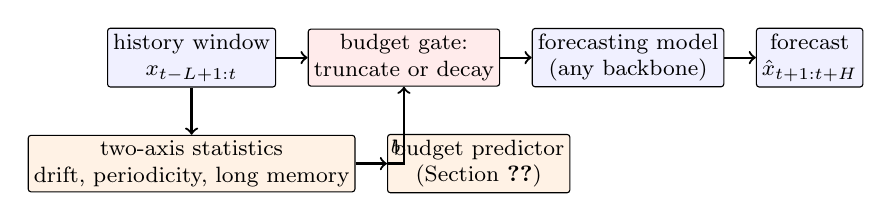
\begin{tikzpicture}[
    font=\footnotesize,
    box/.style={draw, rounded corners=1pt, align=center, minimum height=5.5mm, inner sep=2pt},
    data/.style={box, fill=blue!6},
    comp/.style={box, fill=orange!10},
    gate/.style={box, fill=red!8},
    arr/.style={->, thick},
    lbl/.style={font=\scriptsize\itshape, midway, above}
  ]
  % main path: history -> gate -> model -> forecast
  \node[data] (hist) at (0,0) {history window\\$x_{t-L+1:t}$};
  \node[gate, right=4mm of hist] (gate) {budget gate:\\truncate or decay};
  \node[data, right=4mm of gate] (model) {forecasting model\\(any backbone)};
  \node[data, right=4mm of model] (fcst) {forecast\\$\hat{x}_{t+1:t+H}$};
  % budget path
  \node[comp, below=6mm of hist] (stats) {two-axis statistics\\drift, periodicity, long memory};
  \node[comp, right=4mm of stats] (pred) {budget predictor\\(Section \ref{sec:predictfull})};
  % edges
  \draw[arr] (hist) -- (gate);
  \draw[arr] (gate) -- (model);
  \draw[arr] (model) -- (fcst);
  \draw[arr] (hist.south) -- (stats.north);
  \draw[arr] (stats) -- (pred);
  \draw[arr] (pred) -| node[lbl, pos=0.25] {$b$} (gate.south);
  \end{tikzpicture}
  \caption{History budgeting. Context statistics predict a per-window budget $b$; the input-side gate then either truncates the history to the most recent $b$ steps (hard budget) or weights it by exponential decay with equivalent window $N^*{=}b$ (decay budget, the cross-family default of Section \ref{sec:method}).}
  \label{fig:budget}
\end{figure}

\section{History Budgeting}
\label{sec:method}

The diagnosis of Section \ref{sec:mechanism} says that models do not need a better architecture so much as a controlled supply of history. We introduce \emph{history budgeting}: an input-side module that decides, per window, how much history the model may consume (Figure \ref{fig:budget}).

\paragraph{Design.}
The law of Section \ref{sec:powerlaw} prescribes not only how much history to read but how to weight it: the bias--variance optimum under drift is exponential forgetting \citep{ljung1983}, of which a hard truncation is the zero-order step-function approximation. Each window's effective span $N^* = c\,\hat{\lambda}^{-1/3}$ is computed from its drift index through the calibrated law (with $c{=}65.6$ fitted once on synthetic data), converted to a forgetting factor $\mu = \exp(-1/N^*)$ with a floor $\mu \ge e^{-3/L}$, and applied to the input as $x'(\ell) = x(\ell)\,\mu^{\,t-\ell}$. On the four real benchmarks tested, the raw $N^*$ saturates the floor everywhere, so the auto rule currently reduces to a universal safe decay (recalibration to real drift opposes the synthetic law; Appendix \ref{app:decay}), which remains the recommended default. The module is input-side, adds no parameters, and leaves every backbone unchanged; for zero-shot foundation models the budget is a plain truncation, the only action available to a zero-shot user. Decay never degrades the no-budget baseline in any tested cell (Table \ref{tab:decay} in Appendix \ref{app:decay}), with the largest gains on drift-dominated data (exchange: $-31\%$ on iTransformer, $-59\%$ on PatchTST relative to no budget), though the hard budget remains stronger where zero-fill is admissible (PatchTST on exchange: 0.101 vs.\ 0.164).

\begin{table}[!htb]
\caption{Input-side budget on a trained model (PatchTST, nominal $L{=}2880$, input zeroed beyond the predicted budget $b$, two seeds). The budget run recovers 74--98\% of the gap between the degraded long-window model and the native best-span model, and does not hurt the long-span beneficiary (electricity). Hard input budgeting also dominates the attention-level recency mask (exchange: 0.101 vs.\ 0.263).}
\label{tab:budget}
\centering\scriptsize
\begin{tabular}{lcccc}
\toprule
Dataset ($b$) & No budget @$2880$ & Budget @$2880$ & Native $L{=}b$ & Gap recovered \\
\midrule
Exchange ($96$) & 0.399 & \textbf{0.101} & 0.095 & 98\% \\
ETTh1 ($720$) & 0.623 & \textbf{0.427} & 0.420 & 97\% \\
Weather ($336$) & 0.182 & \textbf{0.160} & 0.153 & 74\% \\
Electricity ($1440$) & 0.130 & 0.128 & 0.129 & no harm \\
\bottomrule
\end{tabular}
\end{table}


\paragraph{Evidence.}
Three results support the design. First, the repair ablation of Section \ref{sec:mechanism} shows that a hard recency mask closes about 45\% of the degradation gap even when applied inside the attention layers, while a learnable null-logit closes nothing; the input-side budget below recovers 74--98\%, so exclusion is most effective on the input path. Second, on a trained model at a fixed nominal window of 2880 steps, zeroing the input beyond the dataset-level budget recovers 74--98\% of the gap to the native best-span model (budgets use the dataset-level measured best span from the iTransformer-side EHS; the statistic predictor of Section \ref{sec:predictfull} places electricity in its saturation plateau and lands within one grid step of the budget on exchange rate and ETTh1) and does not hurt the tested long-span beneficiary, electricity (Table \ref{tab:budget}); the hard input budget also dominates the attention-level recency mask on exchange (0.101 vs.\ 0.263). Third, on a frozen Chronos-Bolt, a dataset-level budget rule (default span 1440, veto to 96 when the context drift index exceeds 0.6) matches validation-based span selection on all eight datasets tested and stays within 0.4\% of the per-dataset oracle, at zero cost (Section \ref{sec:predictfull}, Appendix \ref{app:select}). The threshold merits one caveat: ETT drift indices cluster just below it (ETTh2 0.598, ETTm1 0.525, ETTm2 0.599 on the train-split convention, versus 0.651 for ETTh2 on the full-series convention of Appendix \ref{app:stats}), so the veto is illustrative, not tuned. Two qualifications bound the claim: per-series budgets add almost nothing over dataset-level budgets (the per-series oracle improves on the best fixed span by only 0.2--2.3\%); and decay strength interacts with instance normalization, which rescales the weighted input by the inverse RMS of the weights and amplifies aggressive forgetting, hence the floor and the interior optimum (Appendix \ref{app:decay}).

\paragraph{What the module is not.}
History budgeting is deliberately simple. Like reversible normalization \citep{revin}, which turned a measurement of distribution shift into a one-line fix, the module's role in this paper is to demonstrate that the diagnosis is actionable, not to claim a new modeling family.

\section{Discussion and Conclusion}

\paragraph{Scope.}
Our trained-model measurements cover fourteen public datasets (Appendix \ref{app:ext}), still modest in size and partially criticized for artifacts \citep{fern, timebench}. A GIFT-Eval-scale zero-shot study (25 tasks) shows the law does not transfer to strongly normalized foundation models, where longer context rarely hurts (Appendix \ref{app:gift}); its scope is trained models at benchmark scale. An earlier changepoint-trigger design was removed after resets proved unhelpful (Appendix \ref{app:action}). The full 480-run main matrix carries three seeds per cell (Appendix \ref{app:ledger}). The changepoint formalism assumes abrupt switches, and our two-axis statistics currently handle drift only through the segment-variance index.

\paragraph{What changes for practice.}
For benchmarks, reporting a single fixed lookback conflates model quality with span mismatch; sweeps or budgeted spans should be standard. For foundation models, context length is not a free resource to maximize but a budget to allocate, computable from the context itself. For architecture design, the capacity to suppress stale content determines whether longer context is exploitable at all.

We asked how far back a forecaster should look and found the answer measurable, explainable, and exploitable: the effective history span varies by 30x across problems, is set by the balance of non-stationary cost and regime-invariant benefit, is partially predictable from cheap statistics, and can be enforced by a simple input budget. Lookback is a resource to measure, predict, and spend deliberately.


\bibliographystyle{iclr2027_conference}
\bibliography{refs}

\section*{AI Use Statement}
We used AI-based coding and writing assistants (large language model agents) to help run experiment scaffolding, collate result tables, and copy-edit the manuscript, and an AI-assisted internal review loop to stress-test the claims. All experimental results, numbers, derivations, citations, and scientific claims were produced, executed, and verified by the authors, who take full responsibility for the content of this paper. No AI system was used to generate experimental results or citations without author verification against the primary artifacts.

\section*{Reproducibility Statement}
The measurement protocol, data budgets, per-dataset model configurations, and the complete run ledger (including failed and out-of-memory runs) are documented in Appendices \ref{app:protocol} and \ref{app:ledger}. All analysis scripts, training configurations, and per-run logs are released in the accompanying anonymized code repository; every number in the paper can be traced to a released log or script.

\appendix
\section{Measurement Protocol}
\label{app:protocol}

This appendix specifies the equal-data-budget protocol of Section \ref{sec:measure}: every dataset's training split is capped to the window count available under the longest lookback, and windows are sampled at a fixed stride so that all lookback settings train on exactly the same number of windows. The implementation, sampler, and all launch configurations are released in the accompanying code repository.

\subsection{Equal-data-budget subsampling}

A series whose train split contains $T$ timestamps yields
\begin{equation}
N(T, L, H) \;=\; T - L - H + 1
\end{equation}
overlapping training windows at lookback $L$ and horizon $H$ (we use $H{=}96$ throughout the main matrix). Since $N$ shrinks as $L$ grows, a naive lookback sweep confounds window content with data quantity: the longest lookback trains on the fewest windows. We therefore cap every run of a dataset at the window count of its longest-lookback run,
\begin{equation}
N\_{\min} \;=\; N(T, L\_{\max}, H), \qquad L\_{\max} = 2880,
\end{equation}
and subsample the window \emph{start indices} of every shorter-lookback run down to exactly $N\_{\min}$. Subsampling picks $N\_{\min}$ equally spaced start indices over the full train split via \texttt{np.linspace(0, N-1, N\_min)} followed by rounding and deduplication; it is fully deterministic (no RNG is involved), applies to the train split only, and leaves the validation and test splits untouched. Each run prints \texttt{train window subsample: keep K/N windows}, which we verify against Table \ref{tab:nmin}. When an run's available windows already fit under the cap (e.g.\ exchange rate at $L{=}2880$, where $N = N\_{\min} = 2336$), the sampler is a no-op and the run is identical to an uncapped run. All reported numbers are test MSE/MAE under the standard TSLib evaluation (identity test loader over all test windows).

\subsection{Train-split sizes and \texorpdfstring{$N\_{\min}$}{N min}}

\begin{table}[h]
\caption{Train-split size $T$ (rows), the window-count formula evaluated at $L{=}2880$, $H{=}96$, and the resulting per-run training-window budget $N\_{\min}$ used by every lookback run of the main matrix. ETT borders are fixed calendar splits ($12{\times}30{\times}24$ hours; $4{\times}$ for 15-minute ETTm); the other datasets use the standard TSLib 70/10/20 chronological split. The saturation probe recomputes the budget at $L{=}5760$: $N\_{\min}^{(\mathrm{sat})} = 12557$ (electricity) and $6425$ (traffic).}
\label{tab:nmin}
\centering\small
\begin{tabular}{lcccr}
\toprule
Dataset & Sampling & $T$ (train rows) & Channels & $N\_{\min}$ \\
\midrule
ETTh1, ETTh2 & hourly & 8640 & 7 & 5665 \\
ETTm1, ETTm2 & 15-min & 34560 & 7 & 31585 \\
Exchange & daily & 5311 & 8 & 2336 \\
Weather & 10-min & 36887 & 21 & 33912 \\
Electricity & hourly & 18412 & 321 & 15437 \\
Traffic & hourly & 12280 & 862 & 9305 \\
\bottomrule
\end{tabular}
\end{table}

\subsection{Training protocol and hyperparameters}

All runs share: \texttt{features=M} (multivariate), \texttt{label\_len=48}, \texttt{pred\_len=96}, \texttt{d\_layers=1}, \texttt{factor=3}, Adam optimizer with MSE loss, at most 10 epochs with early stopping (patience 3) on the validation loss, and seeds $\{2021, 2022, 2023\}$. iTransformer and DLinear share one family configuration per dataset (Table \ref{tab:hp_family}); PatchTST and TimesNet use the key hyperparameters of the official TSLib scripts per dataset (Tables \ref{tab:hp_patchtst} and \ref{tab:hp_timesnet}), with the learning rate kept at the official default $10^{-4}$ and TimesNet \texttt{top\_k=5}. These configurations are emitted verbatim by \texttt{gen\_cmds.py} into \texttt{main\_cmds.txt} (480 runs), \texttt{sat\_cmds.txt} (72 saturation runs), and \texttt{remaining\_cmds.txt} (re-run commands for missing runs, with \texttt{OMP\_NUM\_THREADS=2} pinning).

\begin{table}[t]
\caption{Per-dataset configuration shared by iTransformer and DLinear (all with \texttt{n\_heads=8}).}
\label{tab:hp_family}
\centering\small
\begin{tabular}{lccccc}
\toprule
Dataset & $d\_{\mathrm{model}}$ & $d\_{\mathrm{ff}}$ & $e\_{\mathrm{layers}}$ & LR & Batch size \\
\midrule
ETTh1, ETTh2, ETTm1, ETTm2 & 128 & 128 & 2 & $10^{-4}$ & 32 \\
Exchange & 128 & 128 & 2 & $10^{-4}$ & 32 \\
Weather & 512 & 512 & 3 & $10^{-4}$ & 32 \\
Electricity & 512 & 512 & 3 & $5{\times}10^{-4}$ & 16 \\
Traffic & 512 & 512 & 3 & $5{\times}10^{-4}$ & 16 \\
\bottomrule
\end{tabular}
\end{table}

\begin{table}[t]
\caption{PatchTST per-dataset configuration (official TSLib settings; LR $=10^{-4}$ for all).}
\label{tab:hp_patchtst}
\centering\small
\begin{tabular}{lccccc}
\toprule
Dataset & $d\_{\mathrm{model}}$ & $d\_{\mathrm{ff}}$ & $e\_{\mathrm{layers}}$ & Heads & Batch size \\
\midrule
ETTh1 & 512 & 2048 & 1 & 2 & 32 \\
ETTh2 & 512 & 2048 & 3 & 4 & 32 \\
ETTm1 & 512 & 2048 & 1 & 2 & 32 \\
ETTm2 & 512 & 2048 & 3 & 16 & 32 \\
Exchange & 512 & 2048 & 2 & 8 & 32 \\
Weather & 512 & 2048 & 2 & 4 & 32 \\
Electricity & 512 & 2048 & 2 & 8 & 16 \\
Traffic & 512 & 512 & 2 & 8 & 4 \\
\bottomrule
\end{tabular}
\end{table}

\begin{table}[t]
\caption{TimesNet per-dataset configuration (official TSLib settings; LR $=10^{-4}$, \texttt{top\_k=5} for all).}
\label{tab:hp_timesnet}
\centering\small
\begin{tabular}{lccccc}
\toprule
Dataset & $d\_{\mathrm{model}}$ & $d\_{\mathrm{ff}}$ & $e\_{\mathrm{layers}}$ & Heads & Batch size \\
\midrule
ETTh1 & 16 & 32 & 2 & 8 & 32 \\
ETTh2 & 32 & 32 & 2 & 8 & 32 \\
ETTm1 & 64 & 64 & 2 & 8 & 32 \\
ETTm2 & 32 & 32 & 2 & 8 & 32 \\
Exchange & 64 & 64 & 2 & 8 & 32 \\
Weather & 32 & 32 & 2 & 8 & 32 \\
Electricity & 256 & 512 & 2 & 8 & 32 \\
Traffic & 512 & 512 & 2 & 8 & 32 \\
\bottomrule
\end{tabular}
\end{table}

\section{Full Matrices}
\label{app:full}
Per-seed mean$\pm$std tables for all four model families, including cells with partial seed coverage, the saturation probe at $L \in \{2880, 5760\}$, and the Chronos zero-shot sweep.

% Auto-generated by analysis/make_figs.py from logs/ehs_v2/SUMMARY.md,
% logs/ehs_final/taskA_sat.json. Do not edit numbers by hand.
% Requires booktabs and graphicx (for \resizebox).
\begin{table}[t]
\caption{Full lookback sweep for DLinear under the equal-data-budget protocol (test MSE, mean $\pm$ std over seeds 2021--2023; bold = best lookback of the row). All cells aggregate three seeds (Appendix ledger).}
\label{tab:full_dlinear}
\centering\footnotesize
\resizebox{\textwidth}{!}{%
\begin{tabular}{lcccccc}
\toprule
Dataset & $L{=}96$ & $L{=}336$ & $L{=}720$ & $L{=}1440$ & $L{=}2880$ & Best \\
\midrule
ETTh1 & $0.4054\pm0.0009$ & $0.3801\pm0.0003$ & $0.3694\pm0.0003$ & $\mathbf{0.3686}\pm0.0002$ & $0.3907\pm0.0017$ & 1440 \\
ETTh2 & $0.3572\pm0.0035$ & $0.3144\pm0.0017$ & $\mathbf{0.3081}\pm0.0043$ & $0.3132\pm0.0109$ & $0.4530\pm0.0429$ & 720 \\
ETTm1 & $0.3457\pm0.0002$ & $\mathbf{0.3003}\pm0.0003$ & $0.3096\pm0.0023$ & $0.3083\pm0.0003$ & $0.3104\pm0.0002$ & 336 \\
ETTm2 & $0.1919\pm0.0019$ & $0.1694\pm0.0011$ & $0.1634\pm0.0003$ & $0.1621\pm0.0016$ & $\mathbf{0.1619}\pm0.0010$ & 2880 \\
Exchange & $\mathbf{0.1078}\pm0.0021$ & $0.1172\pm0.0014$ & $0.1419\pm0.0048$ & $0.1687\pm0.0216$ & $0.6322\pm0.0101$ & 96 \\
Weather & $0.1961\pm0.0006$ & $0.1753\pm0.0006$ & $0.1695\pm0.0009$ & $0.1677\pm0.0002$ & $\mathbf{0.1673}\pm0.0013$ & 2880 \\
Electricity & $0.1948\pm0.0000$ & $0.1401\pm0.0001$ & $0.1329\pm0.0000$ & $0.1302\pm0.0000$ & $\mathbf{0.1291}\pm0.0000$ & 2880 \\
Traffic & $0.6501\pm0.0001$ & $0.4106\pm0.0000$ & $0.3853\pm0.0001$ & $0.3805\pm0.0000$ & $\mathbf{0.3781}\pm0.0001$ & 2880 \\
\bottomrule
\end{tabular}}
\end{table}

\begin{table}[t]
\caption{Full lookback sweep for PatchTST under the equal-data-budget protocol (test MSE, mean $\pm$ std over seeds 2021--2023; bold = best lookback of the row). All cells aggregate three seeds (Appendix ledger).}
\label{tab:full_patchtst}
\centering\footnotesize
\resizebox{\textwidth}{!}{%
\begin{tabular}{lcccccc}
\toprule
Dataset & $L{=}96$ & $L{=}336$ & $L{=}720$ & $L{=}1440$ & $L{=}2880$ & Best \\
\midrule
ETTh1 & $0.3862\pm0.0028$ & $\mathbf{0.3849}\pm0.0046$ & $0.4017\pm0.0045$ & $0.4567\pm0.0164$ & $0.6228\pm0.0274$ & 336 \\
ETTh2 & $\mathbf{0.2939}\pm0.0016$ & $0.3137\pm0.0057$ & $0.3183\pm0.0045$ & $0.3498\pm0.0179$ & $0.5066\pm0.0524$ & 96 \\
ETTm1 & $0.3266\pm0.0047$ & $\mathbf{0.2911}\pm0.0014$ & $0.3049\pm0.0044$ & $0.3389\pm0.0046$ & $0.3880\pm0.0156$ & 336 \\
ETTm2 & $0.1838\pm0.0027$ & $\mathbf{0.1801}\pm0.0015$ & $0.1851\pm0.0017$ & $0.1911\pm0.0022$ & $0.1934\pm0.0023$ & 336 \\
Exchange & $\mathbf{0.0871}\pm0.0020$ & $0.1048\pm0.0125$ & $0.0924\pm0.0030$ & $0.1385\pm0.0240$ & $0.3804\pm0.0378$ & 96 \\
Weather & $0.1739\pm0.0006$ & $0.1548\pm0.0020$ & $\mathbf{0.1539}\pm0.0023$ & $0.1569\pm0.0046$ & $0.1817\pm0.0079$ & 720 \\
Electricity & $0.1816\pm0.0001$ & $0.1371\pm0.0007$ & $0.1352\pm0.0007$ & $\mathbf{0.1290}\pm0.0007$ & $0.1416\pm0.0088$ & 1440 \\
Traffic & $0.4680\pm0.0003$ & $0.3809\pm0.0008$ & $0.3664\pm0.0007$ & $0.3628\pm0.0004$ & $\mathbf{0.3625}\pm0.0024$ & 2880 \\
\bottomrule
\end{tabular}}
\end{table}

\begin{table}[t]
\caption{Full lookback sweep for TimesNet under the equal-data-budget protocol (test MSE, mean $\pm$ std over seeds 2021--2023; bold = best lookback of the row). All cells aggregate three seeds (Appendix ledger).}
\label{tab:full_timesnet}
\centering\footnotesize
\resizebox{\textwidth}{!}{%
\begin{tabular}{lcccccc}
\toprule
Dataset & $L{=}96$ & $L{=}336$ & $L{=}720$ & $L{=}1440$ & $L{=}2880$ & Best \\
\midrule
ETTh1 & $\mathbf{0.4173}\pm0.0164$ & $0.4261\pm0.0045$ & $0.4356\pm0.0102$ & $0.5736\pm0.0592$ & $1.0904\pm0.1031$ & 96 \\
ETTh2 & $\mathbf{0.3337}\pm0.0022$ & $0.3741\pm0.0250$ & $0.3862\pm0.0072$ & $0.3948\pm0.0191$ & $0.9686\pm0.1439$ & 96 \\
ETTm1 & $\mathbf{0.3326}\pm0.0030$ & $0.3459\pm0.0152$ & $0.3744\pm0.0359$ & $0.3471\pm0.0107$ & $0.4293\pm0.0129$ & 96 \\
ETTm2 & $\mathbf{0.1862}\pm0.0015$ & $0.1879\pm0.0040$ & $0.2130\pm0.0087$ & $0.2392\pm0.0068$ & $0.2116\pm0.0191$ & 96 \\
Exchange & $\mathbf{0.1122}\pm0.0022$ & $0.1643\pm0.0033$ & $0.2919\pm0.0173$ & $0.6894\pm0.2596$ & $2.0699\pm0.3994$ & 96 \\
Weather & $0.1750\pm0.0034$ & $\mathbf{0.1664}\pm0.0035$ & $0.1737\pm0.0037$ & $0.1840\pm0.0033$ & $0.1918\pm0.0047$ & 336 \\
Electricity & $\mathbf{0.1676}\pm0.0011$ & $0.1821\pm0.0027$ & $0.1848\pm0.0037$ & $0.1974\pm0.0065$ & $0.2178\pm0.0037$ & 96 \\
Traffic & $\mathbf{0.5900}\pm0.0046$ & $0.6024\pm0.0066$ & $0.6172\pm0.0042$ & $0.6167\pm0.0033$ & $0.6586\pm0.0060$ & 96 \\
\bottomrule
\end{tabular}}
\end{table}

\begin{table}[t]
\caption{Saturation probe on electricity and traffic with $N_{\min}$ recomputed at $L{=}5760$ (test MSE, mean $\pm$ std). The $L{=}2880$ and $L{=}5760$ arms have three seeds each; shorter arms are single-seed ($^{n1}$). Errors at $L{=}5760$ never improve on $L{=}2880$, so the long-context benefit plateaus instead of being clipped by the scan range.}
\label{tab:sat}
\centering\footnotesize
\resizebox{\textwidth}{!}{%
\begin{tabular}{llcccccc}
\toprule
Dataset & Model & $L{=}96$ & $L{=}336$ & $L{=}720$ & $L{=}1440$ & $L{=}2880$ & $L{=}5760$ \\
\midrule
Electricity & iTransformer & $0.1506\pm0.0000$$^{n1}$ & $0.1329\pm0.0000$$^{n1}$ & $0.1328\pm0.0000$$^{n1}$ & $\mathbf{0.1289}\pm0.0000$$^{n1}$ & $0.1302\pm0.0012$ & $0.1323\pm0.0006$ \\
Electricity & DLinear & $0.1950\pm0.0000$$^{n1}$ & $0.1401\pm0.0000$$^{n1}$ & $0.1330\pm0.0000$$^{n1}$ & $0.1303\pm0.0000$$^{n1}$ & $\mathbf{0.1291}\pm0.0001$ & $0.1294\pm0.0001$ \\
\midrule
Traffic & iTransformer & $0.4127\pm0.0000$$^{n1}$ & $0.3680\pm0.0000$$^{n1}$ & $0.3589\pm0.0000$$^{n1}$ & $0.3554\pm0.0000$$^{n1}$ & $\mathbf{0.3481}\pm0.0019$ & $0.3608\pm0.0006$ \\
Traffic & DLinear & $0.6520\pm0.0000$$^{n1}$ & $0.4114\pm0.0000$$^{n1}$ & $0.3857\pm0.0000$$^{n1}$ & $0.3812\pm0.0000$$^{n1}$ & $\mathbf{0.3787}\pm0.0001$ & $0.3798\pm0.0000$ \\
\bottomrule
\end{tabular}}
\end{table}

\begin{table}[t]
\caption{Zero-shot Chronos-Bolt (single run; test MSE\,/\,MAE). The data-side ordering persists without any training on our corpora: the ETT datasets and weather improve monotonically up to $L{=}1440$, while exchange rate is best at $L{=}96$. `--' marks arms cut by the time budget.}
\label{tab:chronos}
\centering\footnotesize
\resizebox{0.85\textwidth}{!}{%
\begin{tabular}{lccccc}
\toprule
Dataset & $L{=}96$ & $L{=}336$ & $L{=}720$ & $L{=}1440$ & $L{=}2880$ \\
\midrule
ETTh1 & $0.5387/0.4114$ & $0.3890/0.3869$ & $0.3691/0.3787$ & $0.3684/0.3764$ & -- \\
ETTh2 & $0.3825/0.3604$ & $0.2856/0.3341$ & $0.2865/0.3309$ & $0.2745/0.3200$ & -- \\
ETTm1 & $1.0144/0.5723$ & $0.3395/0.3427$ & $0.3208/0.3337$ & $0.3112/0.3271$ & -- \\
ETTm2 & $0.3031/0.3241$ & $0.1828/0.2551$ & $0.1748/0.2484$ & $0.1640/0.2410$ & -- \\
Electricity & -- & -- & -- & -- & -- \\
Exchange & $0.0901/0.2058$ & $0.1080/0.2263$ & $0.1019/0.2239$ & $0.0962/0.2167$ & -- \\
Traffic & -- & -- & -- & -- & -- \\
Weather & $0.6508/0.2939$ & $0.1813/0.2231$ & $0.1691/0.2096$ & $0.1582/0.1977$ & -- \\
\bottomrule
\end{tabular}}
\end{table}


\section{Span Sensitivity and Horizon Robustness}
\label{app:robust}

\subsection{Parsimonious EHS under \texorpdfstring{$\varepsilon$}{eps}}
Table \ref{tab:eps_sens} recomputes the parsimonious effective history span (Eq.\ \ref{eq:ehs}) from the iTransformer sweep means. On drift-dominated datasets with a sharp optimum (exchange, ETTh2, ETTm1/m2, weather) the argmin span $L^*$ and the parsimonious span coincide for all tested $\varepsilon$. On benefit-dominated datasets whose error curve is flat near the optimum they separate: electricity has $L^*{=}2880$ but EHS$(0.02){=}336$, and traffic moves to 1440 at $\varepsilon{=}0.05$ as its near-optimum plateau widens. The separation is diagnostic of how saturated the benefit is; we report $L^*$ in the main text and both conventions here.

\begin{table}[h]
\caption{EHS under Eq.\ \ref{eq:ehs} as a function of the parsimony tolerance $\varepsilon$ (iTransformer sweep means). Parentheses give $L^*$ where it differs.}
\label{tab:eps_sens}
\centering\small
\begin{tabular}{lccc}
\toprule
Dataset & $\varepsilon{=}0.01$ & $\varepsilon{=}0.02$ & $\varepsilon{=}0.05$ \\
\midrule
ETTh1 & 720 & 96 (borderline) & 96 \\
ETTh2 & 96 & 96 & 96 \\
ETTm1 & 336 & 336 & 336 \\
ETTm2 & 336 & 336 & 336 \\
Electricity & 1440 ($L^*{=}2880$) & 336 ($L^*{=}2880$) & 336 ($L^*{=}2880$) \\
Exchange & 96 & 96 & 96 \\
Traffic & 2880 & 2880 (borderline) & 1440 (borderline) \\
Weather & 336 & 336 & 336 \\
\bottomrule
\end{tabular}
\end{table}

\subsection{Horizon robustness (H=192)}
Table \ref{tab:horizon} repeats the sweep at prediction horizon 192 under the same equal-data-budget protocol (iTransformer, two seeds). The short/flat/long classification of each dataset replicates exactly: exchange stays short-optimal, electricity stays long-optimal, ETTh1 stays flat.

\begin{table}[h]
\caption{Test MSE at horizon $H{=}192$ (iTransformer, equal data budget, two seeds). Class labels match the $H{=}96$ sweep.}
\label{tab:horizon}
\centering\small
\begin{tabular}{lcccc}
\toprule
Dataset & $L{=}96$ & $L{=}336$ & $L{=}1440$ & Class \\
\midrule
Exchange & \textbf{0.178} & 0.218 & 0.401 & short \\
ETTh1 & 0.449 & \textbf{0.440} & 0.448 & flat \\
Electricity & 0.165 & 0.154 & \textbf{0.148} & long \\
\bottomrule
\end{tabular}
\end{table}

\section{Extended Suite Sweep}
\label{app:ext}

Six additional public datasets were swept under the identical equal-data-budget protocol (sources and preprocessing are documented in the accompanying repository; the wind candidate was rejected for market-wide block missingness). Table \ref{tab:ext} gives the full matrices; the classification replicates the main suite: five of the six are periodicity-dominated with long or unbounded optimal spans, and the single drift-dominated newcomer (ERCOT settlement prices) is the only one whose iTransformer optimum is short.

\begin{table}[h]
\caption{Equal-budget lookback sweep on the six extension datasets (test MSE, mean $\pm$ std over seeds 2021--2023; bold = best lookback of the row).}
\label{tab:ext}
\centering\footnotesize
\resizebox{\textwidth}{!}{%
\begin{tabular}{llcccccc}
\toprule
Model & Dataset & $L{=}96$ & $L{=}336$ & $L{=}720$ & $L{=}1440$ & $L{=}2880$ & Best \\
\midrule
\multirow{6}{*}{iTransformer}
 & solar & $0.2205{\pm}0.0123$ & $0.2151{\pm}0.0098$ & $0.1868{\pm}0.0045$ & $0.1839{\pm}0.0209$ & $\mathbf{0.1815}{\pm}0.0071$ & 2880 \\
 & PEMS04 & $0.8700{\pm}0.0006$ & $0.6431{\pm}0.0052$ & $0.6582{\pm}0.0016$ & $\mathbf{0.5727}{\pm}0.0073$ & $0.5915{\pm}0.0079$ & 1440 \\
 & PEMS08 & $0.9716{\pm}0.0027$ & $0.7354{\pm}0.0023$ & $0.7266{\pm}0.0094$ & $0.6936{\pm}0.0097$ & $\mathbf{0.6284}{\pm}0.0080$ & 2880 \\
 & bikes & $0.2340{\pm}0.0007$ & $0.2165{\pm}0.0005$ & $0.2145{\pm}0.0003$ & $0.2147{\pm}0.0005$ & $\mathbf{0.2109}{\pm}0.0002$ & 2880 \\
 & pedestrian & $0.3552{\pm}0.0041$ & $0.2370{\pm}0.0007$ & $\mathbf{0.2330}{\pm}0.0004$ & $0.2479{\pm}0.0028$ & $0.2519{\pm}0.0030$ & 720 \\
 & ercot & $0.2249{\pm}0.0007$ & $\mathbf{0.2117}{\pm}0.0011$ & $0.2173{\pm}0.0010$ & $0.2251{\pm}0.0005$ & $0.2278{\pm}0.0015$ & 336 \\
\midrule
\multirow{6}{*}{DLinear}
 & solar & $0.2858{\pm}0.0015$ & $0.2217{\pm}0.0002$ & $0.1906{\pm}0.0000$ & $\mathbf{0.1763}{\pm}0.0002$ & $0.1778{\pm}0.0001$ & 1440 \\
 & PEMS04 & $0.9197{\pm}0.0024$ & $0.7312{\pm}0.0037$ & $0.7313{\pm}0.0026$ & $0.6921{\pm}0.0061$ & $\mathbf{0.5665}{\pm}0.0003$ & 2880 \\
 & PEMS08 & $1.0412{\pm}0.0010$ & $0.8562{\pm}0.0002$ & $0.8381{\pm}0.0015$ & $0.8131{\pm}0.0007$ & $\mathbf{0.6445}{\pm}0.0002$ & 2880 \\
 & bikes & $0.3003{\pm}0.0016$ & $0.2276{\pm}0.0007$ & $0.2213{\pm}0.0002$ & $0.2174{\pm}0.0000$ & $\mathbf{0.2162}{\pm}0.0001$ & 2880 \\
 & pedestrian & $0.4568{\pm}0.0001$ & $0.2387{\pm}0.0000$ & $0.2198{\pm}0.0000$ & $0.2138{\pm}0.0000$ & $\mathbf{0.2125}{\pm}0.0000$ & 2880 \\
 & ercot & $0.2756{\pm}0.0033$ & $0.2370{\pm}0.0013$ & $0.2345{\pm}0.0020$ & $0.2380{\pm}0.0049$ & $\mathbf{0.2312}{\pm}0.0015$ & 2880 \\
\bottomrule
\end{tabular}}
\end{table}

\section{Run Ledger}
\label{app:ledger}

The main matrix is $8 \times 4 \times 5 \times 3 = 480$ runs (8 datasets, 4 model families, lookbacks $L \in \{96, 336, 720, 1440, 2880\}$, seeds $\{2021, 2022, 2023\}$). \textbf{All 480 runs completed}, and every cell in the paper's tables aggregates three seeds. The saturation probe (electricity and traffic, $L \in \{2880, 5760\}$, 2 model families, 3 seeds) completed all 24 of its verdict-bearing runs, plus 16 single-seed reference cells at $L \le 1440$.

\subsection{Provenance: the initially missing 135 runs}

The matrix was not complete at the first snapshot. Of the 480 planned runs, 135 were missing at that point, for execution-environment reasons only; every one was subsequently re-run to completion on idle capacity, and no completed run was ever excluded from the analysis. We keep the original failure classification here for provenance (Table \ref{tab:ledger}):

\begin{itemize}
\item \textbf{GPU memory failures under co-placement (46 runs).} 38 runs raised \texttt{OutOfMemoryError} and 8 raised \texttt{torch.AcceleratorError}, which inspection of the logs shows to be the same CUDA out-of-memory condition reported asynchronously. These failures concentrated exactly where memory pressure was: all 46 were on the three wide datasets (traffic 23, electricity 20, weather 3), and 35 of 46 were PatchTST or TimesNet runs, the two families whose memory footprint grows with channel count and window length. They spanned all lookbacks ($L{=}96$: 9, 336: 10, 720: 8, 1440: 9, 2880: 10), i.e.\ they reflected co-placement contention rather than a lookback effect. Every one of these runs completed on its first attempt once re-run with one job per GPU.
\item \textbf{Time-box cut, never started (65 runs).} When the scheduling time box closed, the remaining queued runs were cut before launch; all 65 were third-seed ($2023$) runs, spread evenly across the four model families (16--17 each).
\item \textbf{Time-box cut, killed mid-run (24 runs).} Arms in flight at the cut (8 with seed 2021, 7 with 2022, 9 with 2023).
\end{itemize}

\begin{table}[t]
\caption{Classification of the 135 initially missing main-matrix runs (all since re-run to completion). The memory class merges \texttt{OutOfMemoryError} (38) and asynchronously reported CUDA OOM surfacing as \texttt{AcceleratorError} (8). All launch configurations are included in the released repository.}
\label{tab:ledger}
\centering\small
\begin{tabular}{llr}
\toprule
Cause class & Where it concentrated & Arms \\
\midrule
GPU memory (OOM $+$ async CUDA OOM) & wide datasets: traffic 23, electricity 20, weather 3 & 46 \\
\quad of which PatchTST / TimesNet & wide-data $\times$ heavy-model cells & 35 \\
\quad of which iTransformer / DLinear & wide datasets only & 11 \\
Time-box cut, never started & all seed 2023 (third-seed runs) & 65 \\
Time-box cut, killed mid-run & mixed seeds (8/7/9 for 2021/2022/2023) & 24 \\
\midrule
Total & & 135 \\
\bottomrule
\end{tabular}
\end{table}

\subsection{Consequences for the reported conclusions}

Completing the matrix moved two cell argmins, both in DLinear and both on cells that previously carried two seeds: ETTh2 ($1440 \to 720$) and ETTm2 ($1440 \to 2880$). Neither touches the paper's ordering claims (the short/long poles are unchanged on every family) or the two-axis analysis; both cells' new values are reflected in Table \ref{tab:bestl}, the predictability targets of Section \ref{sec:predictfull}, and every downstream number. The zero-shot sweep has 8 open runs at $L{=}2880$ on the six non-wide datasets, which are moot because Chronos-Bolt truncates contexts to 2048 steps.

\section{BOCPD Configuration and Falsification Detail}
\label{app:bocpd}

This appendix gives the full configuration behind the changepoint hypothesis test of Section \ref{sec:bocpd}. We further stress-test the falsification in three ways, with all intermediate tables released in the accompanying repository. First, replacing the t-approximate $p$ with exact permutation $p$ values removes the apparent significance of the headline cell ($\rho=-0.67$: exact $p=0.080$; Holm-adjusted $0.399$ over the model family), so we report the falsification as pattern evidence---a consistent negative direction across hazards that flips sign at hazard $1/1000$---rather than as a significance claim. Second, removing calendar seasonality before detection (two variants) does not reverse the counterexample: under phase removal traffic keeps the shortest expected run length alongside the longest optimal lookback across all hazards, and under seasonal differencing its rank weakens to third--fourth shortest while the correlation stays non-positive---so seasonality is not the confound behind it. Third, a changepoint-model-free drift measure (rolling-window mean differences and symmetrized Gaussian KL) recovers the negative drift--span relation independently (iTransformer: $\rho \in [-0.90, -0.79]$, strongest $\rho=-0.902$, Holm-adjusted $p=0.033$).

\subsection{Observation model and inference}

We run Bayesian online changepoint detection \citep{bocpd} per dataset with a Gaussian observation model with \emph{unknown mean and unknown variance}: a Normal--Inverse--Gamma prior ($\kappa_0 = 1.0$) conjugate to the likelihood gives a Student-$t$ predictive at every run length. The run-length posterior is truncated at $r_{\max} = 3000$. The hazard is constant, swept over
\begin{equation}
H \in \{1/50,\; 1/100,\; 1/250,\; 1/500,\; 1/1000\}.
\end{equation}
Inference uses the train split only (borders identical to \texttt{data\_provider}), with up to 24 channels subsampled per dataset, and the reported statistic is the time-averaged posterior expected run length $\mathbb{E}[r]$ after a burn-in of 500 steps.

\paragraph{Why the statistic is $\mathbb{E}[r]$, and a discarded degenerate variant.} Under a constant hazard, the per-step posterior changepoint probability $p(r_t{=}0)$ is identically $H$ by construction (both posterior branches scale with the same predictive mass), so it carries no information about the data; the informative, data-driven quantity is the run-length \emph{distribution}, summarized by $\mathbb{E}[r]$, whose downward resets mark detected changepoints. Our first implementation used the common simplification ``unknown mean, known variance''; under a constant hazard that variant is degenerate in the same sense ($p(r_t{=}0) \equiv H$ is a construction identity) and its $\mathbb{E}[r]$ is almost entirely prior-determined, so the likelihood has no influence. We discarded it and report only the NIG (unknown mean \emph{and} variance) model.

\paragraph{Sanity checks.} Two synthetic controls validate the implementation: (i) i.i.d.\ Gaussian input yields $\mathbb{E}[r] \approx 1740$ and keeps growing toward the truncation $r_{\max}=3000$ (no changepoints detected, as expected); (ii) a piecewise mean-shift input yields $\mathbb{E}[r] \approx 102$ with resets at the injected shifts (changepoints detected).

\subsection{Full $\mathbb{E}[r]$ table and rank correlations}

\begin{table}[t]
\caption{Expected run length $\mathbb{E}[r]$ (time-averaged posterior mean, in steps; ETTm* steps are 15 minutes, others hourly/daily) per hazard level $H$, with the measured best lookback under the equal-data-budget protocol (iTransformer / DLinear) for reference. Electricity and traffic --- the shortest $\mathbb{E}[r]$ at moderate $H$ --- have the \emph{longest} optimal lookbacks, the opposite of the run-length hypothesis.}
\label{tab:bocpd_er}
\centering\small
\begin{tabular}{lccccc cc}
\toprule
Dataset & $H{=}1/50$ & $H{=}1/100$ & $H{=}1/250$ & $H{=}1/500$ & $H{=}1/1000$ & Best $L$ (iTr) & Best $L$ (DLin) \\
\midrule
ETTh1 & 65 & 76 & 90 & 102 & 114 & 720 & 1440 \\
ETTh2 & 234 & 248 & 262 & 271 & 279 & 96 & 720 \\
ETTm1 & 60 & 64 & 68 & 71 & 74 & 336 & 336 \\
ETTm2 & 363 & 377 & 390 & 399 & 407 & 336 & 2880 \\
Exchange & 210 & 215 & 219 & 221 & 223 & 96 & 96 \\
Weather & 291 & 297 & 301 & 303 & 305 & 336 & 2880 \\
Electricity & 53 & 68 & 122 & 234 & 372 & 2880 & 2880 \\
Traffic & 48 & 59 & 87 & 146 & 238 & 2880 & 2880 \\
\bottomrule
\end{tabular}
\end{table}

\begin{table}[t]
\caption{Spearman rank correlation between $\mathbb{E}[r]$ and measured best lookback across the eight datasets ($n{=}8$) per hazard level. No hazard yields a significant negative correlation after exact-permutation and multiple-comparison control, and the iTransformer side is negative at $H{=}1/50$ only under a t-approximation (exact permutation $p=0.080$), so we read the table as pattern evidence: the direction is negative at moderate hazards and flips positive at the most extreme hazard on both families (DLinear $+0.723$, exact $p=0.056$).}
\label{tab:bocpd_spearman}
\centering\small
\begin{tabular}{lccc}
\toprule
$H$ & iTransformer & DLinear & Mean of the two \\
\midrule
$1/50$ & $-0.667$ ($p{\approx}0.028$) & $+0.000$ ($p{\approx}1.000$) & $-0.289$ ($p{\approx}0.459$) \\
$1/100$ & $-0.581$ ($p{\approx}0.081$) & $+0.114$ ($p{\approx}0.778$) & $-0.157$ ($p{\approx}0.698$) \\
$1/250$ & $-0.457$ ($p{\approx}0.208$) & $+0.292$ ($p{\approx}0.455$) & $+0.060$ ($p{\approx}0.882$) \\
$1/500$ & $-0.272$ ($p{\approx}0.489$) & $+0.495$ ($p{\approx}0.163$) & $+0.301$ ($p{\approx}0.439$) \\
$1/1000$ & $+0.111$ ($p{\approx}0.784$) & $+0.723$ ($p{\approx}0.010$) & $+0.615$ ($p{\approx}0.056$) \\
\bottomrule
\end{tabular}
\end{table}

Table \ref{tab:bocpd_er} lists $\mathbb{E}[r]$ for every hazard; Table \ref{tab:bocpd_spearman} the rank correlations. The hypothesis ``effective span tracks posterior expected run length'' fails at every hazard level: the two datasets with the shortest $\mathbb{E}[r]$ at moderate hazards (traffic 87, electricity 122 at $H{=}1/250$) are exactly those whose optimal lookback is longest (2880), while ETTm2 has the longest $\mathbb{E}[r]$ (390) but an optimal lookback of only 336. Regime persistence is therefore not the axis that sets the effective span; the long-context benefit on electricity and traffic comes from strong daily/weekly periodicity that persists across regimes, not from regime duration (Section \ref{sec:why}).

\section{Context Statistics}
\label{app:stats}

This appendix defines the context statistics used in Sections \ref{sec:predict} and \ref{sec:predictfull} as implemented in the accompanying code repository.

\subsection{Common measurement protocol}

Unless stated otherwise, every statistic is computed \emph{per channel} on the \emph{train split} of the raw series (the identical functions are evaluated on a temporary train-only dataset), restricted to the first $n_{\max} = 12000$ rows of that split, so no validation or test information enters any feature in this paper; for datasets with more than 50 channels we draw 50 channels without replacement using \texttt{numpy.default\_rng(0)} (datasets with fewer channels use all of them), and the reported dataset value is the mean across channels. ACF always denotes the Pearson correlation between $x_{1:n-\ell}$ and $x_{\ell+1:n}$ after subtracting the mean; a statistic returns 0 (or NaN for ACF) on degenerate constant inputs ($\mathrm{std} < 10^{-8}$).

\subsection{Definitions}

\paragraph{Drift index.} Split the series into $n_{\mathrm{seg}} = 20$ contiguous segments of (near-)equal length and measure the variance of the segment means relative to the total variance:
\begin{equation}
\mathrm{drift}(x) \;=\; \frac{\mathrm{Var}\big(\{\bar{x}_s\}_{s=1}^{n_{\mathrm{seg}}}\big)}{\mathrm{Var}(x) + 10^{-12}},
\qquad \bar{x}_s = \text{mean of segment } s .
\end{equation}
It is near 0 for stationary level processes and approaches 1 when level shifts dominate the total variance.

\paragraph{Long-lag autocorrelation.} ACF at a lag of one quarter of the (truncated) series length,
\begin{equation}
\mathrm{long\_acf}(x) \;=\; \mathrm{ACF}\big(x,\; \max(1, \lfloor 0.25\, n \rfloor)\big) .
\end{equation}

\paragraph{Detrended spectral periodicity.} Subtract the mean and a least-squares linear trend, take the power spectrum $P = |\mathrm{rFFT}(x_{\mathrm{dt}})|^2$, zero the DC bin $P_0$, and report the peak-to-total power ratio
\begin{equation}
\mathrm{periodicity\_dt}(x) \;=\; \frac{\max_k P_k}{\sum_k P_k + 10^{-12}} .
\end{equation}

\paragraph{Calendar-aligned autocorrelation (differenced).} Remove the mean and linear trend, take a first difference, $x' = \Delta\,\mathrm{detrend}(x - \bar{x})$, and average the ACF at known calendar lags $\mathcal{P}$:
\begin{equation}
\mathrm{calendar\_acf\_diff}(x) \;=\; \frac{1}{|\mathcal{P}|} \sum_{p \in \mathcal{P}} \mathrm{ACF}(x', p),
\end{equation}
with $\mathcal{P}$ per dataset in Table \ref{tab:calendar}. The companion $\mathrm{long\_acf\_diff}$ is the 25\%-lag ACF of the same detrended-and-differenced series $x'$.

\begin{table}[t]
\caption{Calendar period lags $\mathcal{P}$ (in timesteps) aligned to each dataset's sampling rate: the daily and weekly cycles, except exchange rate (business days: one week, one month).}
\label{tab:calendar}
\centering\small
\begin{tabular}{lll}
\toprule
Dataset & Sampling & $\mathcal{P}$ \\
\midrule
ETTh1, ETTh2, Electricity, Traffic & hourly & $[24, 168]$ \\
ETTm1, ETTm2 & 15-min & $[96, 672]$ \\
Weather & 10-min & $[144, 1008]$ \\
Exchange & daily & $[5, 30]$ \\
solar & 10-min & $[144, 1008]$ \\
PEMS04/08 & 5-min & $[288, 2016]$ \\
ERCOT & hourly & $[24, 168]$ \\
pedestrian & hourly & $[24, 168]$ \\
bikes & hourly & $[24, 168]$ \\
\bottomrule
\end{tabular}
\end{table}

\subsection{Measured values}

\begin{table}[t]
\caption{Dataset-level statistic values (channel means) on the eight main benchmarks (top) and the six extension datasets (bottom), measured on the train split under the protocol above. These are the features behind the predictability analysis of Section \ref{sec:predictfull}: drift correlates negatively and $\mathrm{calendar\_acf\_diff}$ positively with the long-context benefit.}
\label{tab:stats_values}
\centering\small
\begin{tabular}{lccccc}
\toprule
Dataset & periodicity\_dt & drift & long\_acf & calendar\_acf\_diff & long\_acf\_diff \\
\midrule
ETTh1 & 0.313 & 0.525 & 0.184 & 0.296 & 0.068 \\
ETTh2 & 0.270 & 0.598 & 0.023 & 0.251 & 0.023 \\
ETTm1 & 0.181 & 0.523 & 0.122 & 0.106 & $-0.005$ \\
ETTm2 & 0.171 & 0.542 & 0.153 & 0.130 & $-0.013$ \\
Exchange & 0.478 & 0.897 & $-0.259$ & 0.001 & 0.011 \\
Weather & 0.146 & 0.275 & 0.048 & 0.061 & 0.001 \\
Electricity & 0.477 & 0.181 & 0.540 & 0.683 & 0.290 \\
Traffic & 0.475 & 0.027 & 0.627 & 0.510 & 0.253 \\
\midrule
solar & 0.364 & 0.033 & 0.176 & 0.234 & $-$0.026 \\
PEMS04 & 0.163 & 0.090 & $-$0.101 & 0.096 & 0.001 \\
PEMS08 & 0.225 & 0.071 & $-$0.261 & 0.163 & $-$0.004 \\
ERCOT & 0.270 & 0.340 & 0.106 & 0.900 & 0.410 \\
pedestrian & 0.506 & 0.010 & 0.697 & 0.649 & 0.151 \\
bikes & 0.202 & 0.016 & 0.371 & 0.258 & 0.041 \\
\bottomrule
\end{tabular}
\end{table}

\subsection{Lessons from the first version (why detrend/difference is mandatory)}

An earlier pilot version of our statistics measured periodicity by the \emph{raw} spectral peak ratio and autocorrelation on the \emph{raw} series, and both were contaminated by drift. A strong trend concentrates low-frequency power in the spectrum, where it masquerades as a periodic peak: exchange rate scored a spurious periodicity of $0.558$ in v1 despite having no meaningful periodic structure (its detrended score is $0.478$, and its calendar-lag ACF after differencing is $\approx 0$). Symmetrically, raw long-lag ACF is inflated by level drift --- a slowly wandering level keeps the series correlated with itself at any lag --- so calendar and long-lag autocorrelations are only meaningful after detrending \emph{and} first differencing. All statistics reported in the paper use the v2 definitions above.

\paragraph{Extension-suite statistics (v3).}
On the enlarged suite (fourteen datasets, twenty-eight samples), the drift index stays the dominant statistic: pooled over the twenty-eight samples it correlates at $-0.654$ with the log-span ($p = 2\times10^{-4}$) and $-0.768$ with the long-context benefit ($p < 10^{-5}$), and at the dataset level ($n{=}14$, the statistically independent units) at $-0.80$ with the log-span ($p = 5\times10^{-4}$) and $-0.85$ with the benefit ($p = 1\times10^{-4}$). The calendar-aligned differenced ACF is directionally consistent but weaker than the pooled view suggested: $+0.366$ ($p=0.056$) over twenty-eight samples, but the two samples per dataset share identical feature values, so the effective units are fourteen; at $n{=}14$ the correlation is $+0.425$ with $p=0.130$, and it does not survive Holm correction across the ten statistic$\times$target tests that Appendix \ref{app:bocpd} applies by the same standard. We therefore report calendar as a supporting descriptor, not an independent axis of significance. Long-lag ACF and detrended spectral periodicity drop below significance because their earlier signal was carried by the electricity and traffic extremes. Full per-dataset values, source notes, and the updated correlation tables are released in the accompanying repository.

\paragraph{Drift-index conventions.}
An earlier version of this analysis computed the statistics on the first 12000 rows of the whole file, which for the shorter datasets includes validation and test spans. The two conventions differ only where the first 12000 rows cross the train boundary (ETTh1 0.450 full-series vs.\ 0.525 train-split; ETTh2 0.651 vs.\ 0.598; exchange rate 0.894 vs.\ 0.897); every dataset whose train split exceeds 12000 rows is identical under both. Switching to the leakage-free train-split convention leaves every correlation direction and the dataset-level significance pattern intact, and the numbers reported in this paper use it throughout; the residual difference matters only near the veto threshold of the Chronos budget rule, which we disclose in Appendix \ref{app:select}.

\section{Attention and Weight Diagnostics}
\label{app:attn}

This appendix reports the mechanism measurements of Section \ref{sec:mechanism}: attention entropy and mass distribution in PatchTST, DLinear weight-decay profiles, and the repair ablation (scripts and per-run data are released in the accompanying repository).

\subsection{PatchTST attention entropy and mass distribution}

We load the trained PatchTST checkpoints ($d_{\mathrm{model}}{=}512$, $e_{\mathrm{layers}}{=}2$, $d_{\mathrm{ff}}{=}2048$) and, in eval mode (dropout off) over the first 8 test batches, record per layer: the per-query mean attention entropy $H$ (also normalized by $\ln S$), the attention mass on the first (oldest) patch (``sink''), and the total mass on the most recent 10\% of patches. Patch count is $S = (L-16)/8 + 2$. Reference points: uniform attention gives $H/\ln S = 1$, recency mass $0.10$, and sink mass $1/S$.

\begin{table}[t]
\caption{Exchange rate, attention statistics per layer (L0/L1 = first/second layer), mean over seeds 2021/2022. Entropy approaches the uniform ceiling as $L$ grows and the sink dissolves from $0.138$ (twice the uniform level $1/S$ at $L{=}96$) to the uniform level $1/S \approx 0.003$, but the recency mass is never diluted below its uniform share.}
\label{tab:attn_exchange}
\centering\small
\begin{tabular}{cc cccc cc cc}
\toprule
$L$ & $S$ & $H$(L0) & $H/\ln S$(L0) & $H$(L1) & $H/\ln S$(L1) & sink L0 & sink L1 & near-10\% L0 & near-10\% L1 \\
\midrule
96 & 12 & 1.92 & 0.77 & 2.09 & 0.84 & 0.138 & 0.127 & 0.127 & 0.103 \\
720 & 90 & 4.18 & 0.93 & 4.07 & 0.90 & 0.021 & 0.015 & 0.124 & 0.087 \\
2880 & 360 & 5.19 & 0.88 & 5.38 & 0.91 & 0.007 & 0.004 & 0.163 & 0.145 \\
\bottomrule
\end{tabular}
\end{table}

\begin{table}[t]
\caption{Electricity, attention statistics, measured on fully trained uncapped vanilla control runs (Appendix repair ablation, \texttt{none} variant), since the capped $L{\ge}1440$ checkpoints of the main matrix were lost to OOM. Dilution is \emph{stronger} than on exchange rate ($H/\ln S$ at L1 reaches 0.95), yet electricity is where long context helps most.}
\label{tab:attn_electricity}
\centering\small
\begin{tabular}{cc cc cc cc}
\toprule
$L$ & $S$ & $H/\ln S$(L0) & $H/\ln S$(L1) & sink L0 & sink L1 & near-10\% L0 & near-10\% L1 \\
\midrule
96 & 12 & 0.59 & 0.66 & 0.086 & 0.080 & 0.063 & 0.063 \\
1440 & 180 & 0.66 & 0.91 & 0.008 & 0.005 & 0.185 & 0.093 \\
2880 & 360 & 0.75 & 0.95 & 0.003 & 0.003 & 0.192 & 0.129 \\
\bottomrule
\end{tabular}
\end{table}

On the capped main-matrix checkpoints, electricity at $L{=}96$ shows $H/\ln S = 0.60/0.68$ and near-10\% mass $0.063/0.068$ (below the uniform $0.083$); a partially trained $L{=}720$ checkpoint shows $0.77/0.88$ and $0.190/0.114$. Two findings follow. First, softmax dilution is real and universal: normalized entropy rises toward the uniform ceiling on both datasets, and no attention sink survives at long lookbacks. Second, dilution is not harmful by itself: it is stronger on electricity, which benefits from long context, and the recency mass is not diluted on either dataset (exchange $0.13 \to 0.16$, electricity L0 $0.06 \to 0.19$). Whether flattening hurts depends on whether the diluted far content is noise (exchange) or periodic structure (electricity) --- consistent with the DLinear evidence next.

\subsection{DLinear weight profiles}

DLinear learns a linear map per decomposition branch; averaging $|w|$ over output positions gives a mass profile over lag positions (index $0$ = oldest). Table \ref{tab:dlinear} reports, at $L{=}2880$: the mass on the most recent 96 lags, the mass beyond lag 720, and the daily-harmonic contrast (peak power at the daily period relative to its spectral neighborhood).

\begin{table}[t]
\caption{DLinear weight-mass distribution at $L{=}2880$. On exchange rate the seasonal branch places only $6.0\%$ of its mass on the recent 96 lags and $72.6\%$ beyond lag 720 with no periodic structure (contrast $\approx 1$): the linear model does not learn implicit gating, and the diffuse far-lag mass coincides with the $L{=}2880$ degradation (MSE $0.636$). On electricity the far mass is equally large but carries daily/weekly spikes (contrast $1.25$; at $L{=}96$ the seasonal profile shows sharp $d{\approx}24/168$ peaks with contrast $1.67$), and long context helps (MSE $0.129$).}
\label{tab:dlinear}
\centering\small
\begin{tabular}{llccc}
\toprule
Dataset & Branch & Mass(last 96 lags) & Mass(lag $> 720$) & Daily contrast \\
\midrule
Exchange & Linear\_Seasonal & 0.060 & 0.726 & 1.03 \\
Exchange & Linear\_Trend & 0.238 & 0.556 & 1.05 \\
Electricity & Linear\_Seasonal & 0.187 & 0.487 & 1.25 \\
Electricity & Linear\_Trend & 0.181 & 0.529 & 0.94 \\
\bottomrule
\end{tabular}
\end{table}

\subsection{Repair ablation (attention-side fixes)}

We test two attention-internal repairs on PatchTST (\texttt{PatchTSTGated}, an SDPA re-implementation whose \texttt{none} variant is numerically equal to PatchTST, smoke-tested at $\max|\Delta| = 9.5{\times}10^{-7}$): \texttt{denbias}, a learnable off-by-one null logit that lets softmax attend to ``nothing'', and \texttt{recmask}, a hard recency mask (identity at $L{=}96$, where the patch count $12$ is below the mask window). Protocol: exchange rate and electricity $\times$ $L \in \{96, 1440, 2880\}$ $\times$ variant $\times$ seeds $\{2021, 2022\}$, uncapped windows, main-matrix hyperparameters ($d_{\mathrm{model}}{=}512$, $d_{\mathrm{ff}}{=}2048$, $e_{\mathrm{layers}}{=}2$, 8 heads, LR $10^{-4}$; batch size 32 on exchange, $16/8/4$ on electricity for $L = 96/1440/2880$).

\begin{table}[t]
\caption{Repair ablation, test MSE (mean $\pm$ std over seeds 2021/2022). The hard recency mask recovers $34\%$ of the exchange-rate degradation at $L{=}2880$ ($0.399 \to 0.263$, closing $\sim$45\% of the gap to short lookbacks) without hurting electricity; the learnable softmax exit is never used (its null logit stays at $\approx 0$ and the null mass stays $\le 0.4\%$ on exchange), so \texttt{denbias} is pointwise identical to the control. Sanity checks: \texttt{none} at $L{=}2880$ reproduces the capped main-matrix run ($0.399$ vs.\ $0.405$; that run's window count equals the uncapped one), and \texttt{recmask} at $L{=}96$ is bitwise identical to \texttt{none}.}
\label{tab:repair}
\centering\small
\begin{tabular}{lcccc}
\toprule
Dataset / $L$ & none (control) & denbias & recmask & capped PatchTST \\
\midrule
Exchange / 96 & $0.0950\pm0.0009$ & $0.0952\pm0.0010$ & $0.0950\pm0.0009$ & $0.0871\pm0.0020$ \\
Exchange / 1440 & $0.1371\pm0.0003$ & $0.1387\pm0.0030$ & $0.1282\pm0.0132$ & $0.1484\pm0.0239$ \\
Exchange / 2880 & $0.3989\pm0.0168$ & $0.3989\pm0.0181$ & $\mathbf{0.2625\pm0.0424}$ & $0.4053\pm0.0169$ \\
\midrule
Electricity / 96 & $0.1803\pm0.0002$ & $0.1803\pm0.0002$ & $0.1803\pm0.0002$ & $0.1816\pm0.0001$ \\
Electricity / 1440 & $0.1291\pm0.0003$ & $0.1285\pm0.0003$ & $0.1291\pm0.0003$ & -- (OOM) \\
Electricity / 2880 & $0.1301\pm0.0009$ & $0.1384\pm0.0089$ & $\mathbf{0.1269\pm0.0000}$ & -- (OOM) \\
\bottomrule
\end{tabular}
\end{table}

About half of the long-context harm on exchange rate is directly attributable to attention being forced to read the entire far past (a hard mask recovers it); the remainder sits in the value/head pathway (on electricity at $L{=}2880$ the vanilla validation curve oscillates violently while \texttt{recmask}/\texttt{denbias} converge smoothly, indicating an optimization component). A learnable softmax exit is not an effective mechanism --- gradients never use it. (The \texttt{denbias} outlier on electricity at $L{=}2880$ is single-seed noise: seed 2022 early-stopped after epoch 1 at $0.1473$ while seed 2021 reached $0.1295$.)

\section{Latent-Action Probes}
\label{app:action}
We probed a stronger version of the trigger idea in which shocks are discovered unsupervised as discrete latent actions with a quantized bottleneck. Two rounds of controlled experiments on synthetic shock data show that the bottleneck does route shock effects through the discrete codes and supports counterfactual intervention (intervening on the code moves the forecast toward the counterfactual by 16.5\% on fired events), but that type-level semantics do not emerge without supervision (NMI ceiling 0.23), and that pointwise surprise triggers cannot see trend- or frequency-level changes (recall below 0.1). A follow-up demonstration with an accumulated-evidence (CUSUM-style) trigger closes this design branch: detection improves only for frequency-type shocks (recall 0.11 $\to$ 0.31) while trend shocks remain invisible (0.08), and resetting the budget at detected or even oracle shock times consistently degrades prediction (component-level shocks leave other components predictable from the past, so forgetting costs exceed staleness benefits). We therefore removed the trigger from the method design. The full protocol and metrics are released in the accompanying repository.

\subsection{Setup}

Synthetic series of length 512 (random trend + 1--3 harmonics + AR(2) noise) are injected with 0--3 shocks of four types: \emph{level} (mean step), \emph{vol} (noise-std step), \emph{trend} (slope step), and \emph{freq} (dominant-harmonic frequency step, phase-continuous), with a shock-free counterfactual of the same base series. The probe model is a patch transformer (patch 16, $d_{\mathrm{model}}{=}128$, 4-layer causal encoder, 2-layer causal decoder, 96-step forecast) whose 3-dim action head is quantized by FSQ (levels $[5,5,5]$, 125 codes) and, under the \emph{action bottleneck}, is the only channel through which patch $i$'s information enters the prediction ($z_{i-1} + \mathrm{up}(q_i)$). Alignment metrics: an \emph{event} is a code change between adjacent patches; a shock is \emph{hit} (recall) if an event fires within $\pm 1$ patch of it; \emph{precision} is the fraction of events that hit a shock (chance $\approx 0.145$); NMI and \emph{purity} (chance $0.25$) relate fired codes to shock types.

\subsection{Round 1: the bottleneck is necessary but not sufficient}

\begin{table}[t]
\caption{Round-1 alignment metrics (validation, 2048 series). Without the bottleneck the code drifts with the continuous state (precision at chance); the bottleneck forces reliable firing (recall up to 0.99) but precision stays at chance and type semantics are weak (NMI $\le 0.105$), because the code is hijacked into digitizing the continuous state trajectory.}
\label{tab:action_v1}
\centering\small
\begin{tabular}{llccccc}
\toprule
Configuration & Regime & Events/seq & Recall & Precision & NMI & Purity \\
\midrule
FSQ, no bottleneck & standard & 20.5 & 0.922 & 0.147 & 0.019 & 0.307 \\
FSQ + bottleneck & standard & 28.9 & 0.982 & 0.144 & 0.036 & 0.381 \\
FSQ + bottleneck, TV-L1 0.03 & quiet & 19.5 & 0.937 & 0.166 & 0.105 & 0.489 \\
\bottomrule
\end{tabular}
\end{table}

The bottleneck costs only $+1.3\%$ prediction MSE, and intervening on the fired code (swapping in the calm-sequence mode code) raises the error against the true post-shock series by $+29\%$ (level $+61\%$, trend $+65\%$, vol $+25\%$, freq $+17\%$) while moving it only $-5\%$ toward the shock-free counterfactual: shock responses are partially routed through the codes, but single-token swaps cannot erase a shock, and semantics remain diffuse.

\subsection{Round 2: innovation coding, a reserved null code, and NLL}

Round 2 feeds the code the \emph{innovation} (residual of the patch against a detached predictor) instead of the encoder state, reserves code 0 as a null ``no-event'' code with gated firing (whitened-surprise threshold $\tau = c \times$ EMA-RMS), and optionally trains with Gaussian NLL so that volatility shocks pay off in likelihood.

\begin{table}[t]
\caption{Round-2 alignment metrics (standard regime; v1 bottleneck row for reference). Sparsification moves precision off its chance level only with \emph{absolute} thresholds (gt1.5/gt2.0), and the best semantics (NMI $0.226$, purity $0.694$, configuration M: MLP predictor + rich features + 2-patch accumulation) remain far from clean type discovery; the precision ceiling $0.371$ is reached at recall $0.17$. Quantile-forced gating pins precision to chance by construction; NLL never helps firing.}
\label{tab:action_v2}
\centering\small
\begin{tabular}{lccccccc}
\toprule
Configuration & MSE & Events/seq & Null \% & Recall & Precision & NMI & Purity \\
\midrule
FSQ + bottleneck (v1) & 0.538 & 28.9 & -- & 0.98 & 0.144 & 0.036 & 0.381 \\
\quad + innovation input (A) & 0.546 & 28.7 & -- & 0.98 & 0.144 & 0.044 & 0.396 \\
\quad + null, quantile 0.85 white (G) & 0.578 & 8.1 & 0.85 & 0.61 & 0.202 & 0.105 & 0.498 \\
\quad + white threshold 1.5 (L) & 0.587 & 3.9 & 0.93 & 0.42 & 0.260 & 0.137 & 0.559 \\
\quad + white threshold 2.0 (J) & 0.591 & 1.0 & 0.98 & 0.17 & \textbf{0.371} & 0.185 & 0.690 \\
\quad J + MLP pred.\ + accum (M) & 0.595 & 0.6 & 0.99 & 0.09 & 0.343 & \textbf{0.226} & \textbf{0.694} \\
\quad M + NLL (O) & 0.619 & 0.6 & 0.99 & 0.08 & 0.342 & 0.223 & 0.653 \\
\bottomrule
\end{tabular}
\end{table}

Three findings carry into the main-text design. \textbf{(i) Intervention gets cleaner under sparsity.} Restricting to events where the gate actually fired, swapping in the null code moves the prediction toward the shock-free counterfactual by $-16.5\%$ (J: $0.746 \to 0.623$) and $-17\%$ (M: $0.860 \to 0.716$), while error against the true series rises by $+6\%$/$+9\%$ --- once a code fires, the shock response is carried mainly by that code. \textbf{(ii) Pointwise surprise has a hard ceiling.} At the sparse thresholds, per-type recall for \emph{trend} and \emph{freq} shocks collapses to $0.03$--$0.09$ (e.g.\ J: $0.041/0.070$; M: $0.026/0.040$): slope and phase changes are accumulated evidence, invisible to single-patch surprise. This motivated an accumulated-evidence trigger, which our follow-up demonstration (below) later vetoed, and the component was removed from the method design. \textbf{(iii) The remaining ceilings are structural.} Type--magnitude entanglement caps purity at $\approx 0.69$; quantile-forced trigger rates cap precision near chance; and NLL removes the incentive to route vol through the code (the variance head absorbs it). Unsupervised discovery of shock \emph{types} therefore needs explicit weak supervision or a semantics-friendly loss, which we leave to future work.

\section{Span-Selection Baselines}
\label{app:select}

This appendix details the four span selectors compared in Section \ref{sec:predictfull} (scripts and full per-cell tables are released in the accompanying repository).

\subsection{Selector definitions}

\paragraph{Statistic predictor (ours).} The leave-one-dataset-out ridge predictor of Section \ref{sec:predictfull} ($k{=}3$ features selected inside each fold by $|\rho|$, predicting $\log_2 L^*$ and rounding to the nearest grid point), computed from train-split statistics. A single $n{=}28$ LOO regressor produces the predictions for both the sixteen main-suite cells and the pooled twenty-eight-cell view of Section \ref{sec:predictfull}; the two rows in Table \ref{tab:selectors} differ only in which cells they aggregate.

\paragraph{Validation selection (standard HPO).} For each run we parse the per-epoch validation loss (the early-stopping criterion) and take its minimum as that run's validation error; the selected lookback minimizes the seed-averaged validation error. All 32 dataset$\times$model rows (four families) parsed successfully. A per-seed variant (select per seed, then average) gives an almost identical mean regret ($+0.0036$ vs.\ $+0.0027$ MSE).

\paragraph{PACF last-significant-lag.} On the train split ($\le 32$ channels, seed-0 subsample), ACF (FFT, max lag 2880) is computed and Levinson--Durbin recursion yields the PACF; the suggested order is the largest lag outside the 95\% band, mapped to the nearest grid point on the $\log_2$ scale.

\paragraph{AIC order.} From the same recursion, the AR($p$) innovation variance gives $\mathrm{AIC}(p) = N \log \hat{\sigma}^2(p) + 2p$ (the Yule--Walker construction of R's \texttt{ar(aic=TRUE)}); the argmin order is mapped to the grid as above.

\subsection{Results on the trained matrix}

\begin{table}[t]
\caption{Selector comparison on the 16 dataset$\times$model cells of the main suite (8 datasets $\times$ \{iTransformer, DLinear\}): exact hits against the test oracle, mean absolute and relative test-MSE regret, and selection cost. Under the leakage-free train-split convention the statistic predictor no longer matches validation selection for trained models. PACF degenerates to always picking 2880; its six exact hits are exactly the cells right-censored at the scan ceiling, and its misses are catastrophic (exchange rate $+261\%$/$+489\%$ relative). Per-cell values are included in the released run ledger.}
\label{tab:selectors}
\centering\footnotesize
\begin{tabular}{lcccc l}
\toprule
Selector & Exact hit & Mean regret & Mean rel.\ & Median rel.\ & Cost \\
\midrule
Statistic predictor ($k{=}3$ LOO) & 3/16 & $+0.0075$ & $+4.52\%$ & $+2.30\%$ & $\approx 0$ (3 statistics) \\
Validation selection & \textbf{8/16} & \textbf{$+0.0031$} & \textbf{$+1.01\%$} & \textbf{$+0.07\%$} & 5 spans $\times$ full training \\
AIC order $\to$ grid & 2/16 & $+0.0080$ & $+3.49\%$ & $+2.91\%$ & low \\
PACF last sig.\ lag $\to$ grid & 6/16 (degenerate) & $+0.0786$ & $+57.8\%$ & $+10.09\%$ & low \\
\midrule
\multicolumn{6}{l}{\emph{Pooled extension suite (14 datasets $\times$ 2 families $=$ 28 cells)}} \\
Statistic predictor ($k{=}3$ LOO) & 8/28 & --- & $+5.33\%$ & $+2.30\%$ & $\approx 0$ \\
Validation selection & \textbf{16/28} & --- & \textbf{$+0.92\%$} & \textbf{$+0.00\%$} & 5 spans $\times$ full training \\
\bottomrule
\end{tabular}
\end{table}

Two distinct pools appear in this paper and should not be conflated: the \emph{pooled extension suite} above (fourteen datasets $\times$ two families, used for the headline comparison of Section \ref{sec:predictfull}), and the \emph{four-family main grid} (eight datasets $\times$ four model families $=$ 32 cells, all complete). Both statistic-predictor rows come from the same $n{=}28$ LOO regressor, so their difference reflects only the aggregated cells, not a refit. Validation selection on the four-family grid hits the oracle in 20/32 cells with mean relative regret $0.86\%$ (median $0.00\%$). Its failure modes are systematic: (a) long-window benefit that has not yet surfaced on the validation split (traffic/iTransformer: validation picks 720, oracle 2880, $+5.1\%$), (b) the symmetric short-window miss (ETTh2/PatchTST: validation picks 336, oracle 96, $+6.8\%$), and (c) weak resolution between adjacent grid points on ETT (ETTh1/iTransformer: validation picks 96 vs.\ oracle 720, $+2.0\%$).

\begin{table}[t]
\caption{PACF/AIC classical order selection: channel-median orders on level and first-differenced train series, mapped to the lookback grid, against the measured best lookback. PACF's significant lags extend to the 2880 cap on all eight datasets (a known long tail for strongly periodic series), so it always proposes 2880; AIC orders carry structure but measure only short-range linear predictability.}
\label{tab:pacf_aic}
\centering\footnotesize
\resizebox{\textwidth}{!}{%
\begin{tabular}{lcccc cc}
\toprule
Dataset & PACF order (level/diff) & $\to$ grid & AIC order (level/diff) & $\to$ grid & Best $L$ (iTr) & Best $L$ (DLin) \\
\midrule
ETTh1 & 2796 / 2812 & 2880 & 222 / 221 & 336 & 720 & 1440 \\
ETTh2 & 2766 / 2765 & 2880 & 266 / 265 & 336 & 96 & 720 \\
ETTm1 & 2874 / 2873 & 2880 & 598 / 675 & 720 & 336 & 336 \\
ETTm2 & 2876 / 2875 & 2880 & 677 / 676 & 720 & 336 & 2880 \\
Exchange & 2281 / 2445 & 2880 & 10 / 16 & 96 & 96 & 96 \\
Weather & 2872 / 2871 & 2880 & 169 / 297 & 96 / 336 & 336 & 2880 \\
Electricity & 2857 / 2857 & 2880 & 516 / 510 & 720 & 2880 & 2880 \\
Traffic & 2854 / 2856 & 2880 & 506 / 505 & 720 & 2880 & 2880 \\
\bottomrule
\end{tabular}}
\end{table}

\paragraph{Validation-window caveat.} In the standard TSLib protocol the number of validation windows varies with lookback, so each candidate's validation MSE is computed on a slightly different target set. We deliberately apply no correction for this: the variable-window validation set \emph{is} standard practice, and what we evaluate is that practice as-is. The per-seed selection variant changes the mean regret by only $0.0001$ MSE.

\subsection{Zero-shot selector (Chronos-Bolt)}

Chronos-Bolt has no training and no canonical validation usage, so we split the cached per-window test errors temporally: the first 50\% of windows serves as the selection set, the last 50\% as the evaluation set, at zero re-inference cost (electricity uses the stride-2 subsampled cache, internally fair across lookbacks).

\begin{table}[t]
\caption{Zero-shot span selection on Chronos-Bolt (evaluation on the temporally later 50\% of test windows). The dataset-level statistic rule (default 1440, veto to 96 when the dataset-mean drift index exceeds $0.6$) selects the \emph{same} lookback as validation selection on all eight datasets, at zero cost. Per-channel selection is worse than dataset-level selection on 2 of 4 datasets (selection noise), supporting that the exploitable gain lives at the dataset level.}
\label{tab:select_chronos}
\centering\footnotesize
\begin{tabular}{lccc ccc cc}
\toprule
Dataset & Val-sel.\ $L$ & Oracle $L$ & Hit & MSE (val-sel) & MSE (rule) & MSE (oracle) & Regret (val) & Regret (rule) \\
\midrule
ETTh1 & 1440 & 720 & n & 0.4205 & 0.4205 & 0.4192 & $+0.0013$ & $+0.0013$ \\
ETTh2 & 1440 & 1440 & Y & 0.3530 & 0.3530 & 0.3530 & $+0.0000$ & $+0.0000$ \\
ETTm1 & 1440 & 1440 & Y & 0.3549 & 0.3549 & 0.3549 & $+0.0000$ & $+0.0000$ \\
ETTm2 & 1440 & 1440 & Y & 0.2105 & 0.2105 & 0.2105 & $+0.0000$ & $+0.0000$ \\
Exchange & 96 & 96 & Y & 0.0949 & 0.0949 & 0.0949 & $+0.0000$ & $+0.0000$ \\
Weather & 1440 & 1440 & Y & 0.1474 & 0.1474 & 0.1474 & $+0.0000$ & $+0.0000$ \\
Electricity & 1440 & 720 & n & 0.1203 & 0.1203 & 0.1202 & $+0.0002$ & $+0.0002$ \\
Traffic & 1440 & 1440 & Y & 0.4178 & 0.4178 & 0.4178 & $+0.0000$ & $+0.0000$ \\
\bottomrule
\end{tabular}
\end{table}

The rule and validation selection coincide exactly on 8/8 datasets, and the two oracle misses are harmless (the zero-shot error surface is flat between 1440 and 720, $<0.4\%$). The coincidence is partly structural: the default 1440 arm is itself validation-optimal on six of the eight datasets, so the discriminative content of the rule is the exchange-rate veto, and the oracle comparison (two misses, both $<0.4\%$) bounds what either method leaves on the table. The veto threshold, however, sits in a dense region of ETT drift indices: on the train-split convention used by the budgeting chain, ETTh1 0.525, ETTh2 0.598, ETTm1 0.525, and ETTm2 0.599 all land just below the $0.6$ veto, while ETTh2's full-series value ($0.651$, Appendix \ref{app:stats}) would cross it. Every ETT dataset genuinely prefers 1440 in this zero-shot study, so the rule is correct on them either way; the threshold should nevertheless be read as illustrative rather than tuned.

\begin{figure}[t]
  \centering
  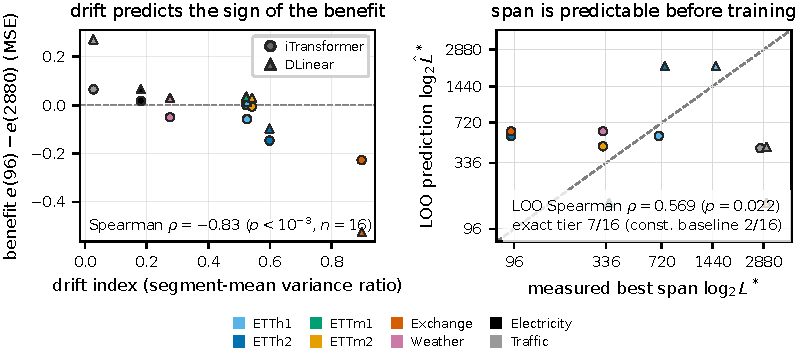
\includegraphics[width=0.52\linewidth]{figs/fig2_predictability.pdf}
  \caption{The effective span is predictable from training-free context statistics computed on the train split only. Left: drift index versus measured long-context benefit across the eight main-suite benchmarks and two model families (Spearman $\rho = -0.83$ over the sixteen samples; cluster-level reading over the eight datasets $\rho = -0.88$, $p = 0.004$). Right: leave-one-dataset-out predicted versus measured log-span (main-suite panel; the enlarged fourteen-dataset suite of Section \ref{sec:predictfull} gives $\rho = 0.63$; dashed line is identity).}
  \label{fig:predict}
\end{figure}


\section{The Power-Law Experiment}
\label{app:powerlaw}

This appendix specifies the controlled synthetic test of the bias--variance law $W^* \propto \lambda^{-2/3}$ behind Section \ref{sec:powerlaw} (generator, sweep configuration, fitting code, and all per-tier numbers are released in the accompanying repository).

\subsection{Generator and drift-rate calibration}

Each channel is an independent Poisson shock process: shocks arrive with probability $\lambda$ per step (so run lengths are geometric and $\mathbb{E}[\text{run}] = 1/\lambda$ exactly), each shock is a level step of amplitude $U(0.8, 2.0)$ with random sign (pure drift, no periodic component), on top of AR(1) base noise ($a{=}0.3$) with marginal $\sigma = 12$ (about $8\times$ the RMS step size). Series have $T{=}25000$ steps (train 17500 / validation 2500 / test 5000) and 4 channels. The sweep spans six nominal drift rates, $\mathbb{E}[r] \in \{50, 150, 400, 1000, 2500, 6000\}$.

The high noise ratio is a load-bearing design choice. A first version with $\sigma{=}1$ (archived in the released logs) put the bias--variance optimum below the scan range for every $\lambda$: all $W^*$ were censored at the grid boundary $96$/$192$, and no exponent could be measured. Raising $\sigma$ to $12$ moves the optimum into the interior of $\{96, \dots, 2880\}$.

\begin{table}[t]
\caption{Drift-rate calibration: nominal expected run length, shock probability $\lambda$, measured expected run length, and the resulting drift index (Appendix \ref{app:stats}, $n_{\mathrm{seg}}{=}20$), mean $\pm$ std over 30 realizations $\times$ 4 channels. $\lambda$ maps strictly monotonically onto the measured drift index (adjacent levels are separated by 4--8 standard errors), and measured $\mathbb{E}[r]$ tracks the $1/\lambda$ diagonal. The periodic variants sit slightly below the pure-drift run at the same $\lambda$ (periodic energy inflates the denominator), which does not affect the $\lambda$ axis.}
\label{tab:calibration}
\centering\small
\begin{tabular}{cccc}
\toprule
Nominal $\mathbb{E}[r]$ & $\lambda$ & Measured $\mathbb{E}[r]$ & Drift index \\
\midrule
50 & 0.020 & 50 & $0.3854 \pm 0.0173$ \\
150 & 0.0067 & 160 & $0.1881 \pm 0.0118$ \\
400 & 0.0025 & 429 & $0.0897 \pm 0.0069$ \\
1000 & 0.0010 & 885 & $0.0402 \pm 0.0029$ \\
2500 & 0.0004 & 2659 & $0.0160 \pm 0.0013$ \\
6000 & 0.00017 & 5312 & $0.0087 \pm 0.0007$ \\
\bottomrule
\end{tabular}
\end{table}

\subsection{Sweep protocol and the \texorpdfstring{$\lambda \times L$}{lambda x L} error surface}

We train a small iTransformer ($d_{\mathrm{model}}{=}64$, $d_{\mathrm{ff}}{=}64$, $e_{\mathrm{layers}}{=}2$, 8 heads, batch 64, LR $10^{-3}$, at most 5 epochs with patience-3 early stopping, horizon 96) over lookbacks $L \in \{96, 192, 336, 720, 1440, 2880\}$ and seeds $\{2021, 2022\}$, all runs under the equal-data-budget protocol with $N_{\min} = 14525$ training windows (the count of the $L{=}2880$ run).

\begin{table}[t]
\caption{Test MSE (2-seed mean) on the pure-drift sweep; bold marks the grid argmin $W^*$. Every level shows an interior U-shaped minimum. Per-seed argmins agree on 5 of 6 levels (at \texttt{er6000} the curve is near-flat, adjacent cells differ by $\sim 2{\times}10^{-4}$, and the two seeds split between 1440 and 2880).}
\label{tab:error_surface}
\centering\small
\begin{tabular}{lcccccc c}
\toprule
Dataset & 96 & 192 & 336 & 720 & 1440 & 2880 & $W^*$ (grid) \\
\midrule
drift\_er50 & 0.4794 & 0.4785 & \textbf{0.4783} & 0.4798 & 0.4823 & 0.4901 & 336 \\
drift\_er150 & 0.7702 & 0.7650 & \textbf{0.7644} & 0.7663 & 0.7665 & 0.7742 & 336 \\
drift\_er400 & 0.8978 & 0.8907 & \textbf{0.8889} & 0.8890 & 0.8907 & 0.8918 & 336 \\
drift\_er1000 & 0.9898 & 0.9819 & 0.9800 & \textbf{0.9794} & 0.9828 & 0.9821 & 720 \\
drift\_er2500 & 0.9951 & 0.9871 & 0.9849 & \textbf{0.9832} & 0.9836 & 0.9847 & 720 \\
drift\_er6000 & 1.0086 & 1.0004 & 0.9979 & 0.9961 & \textbf{0.9958} & 0.9959 & 1440 \\
\bottomrule
\end{tabular}
\end{table}

\subsection{Fitting conventions and verdict}

We fit $\ln W^*$ against $\ln \lambda$ by OLS under two conventions: the grid argmin above, and a parabolic interpolation of the error curve around the argmin (sensitivity analysis), giving interpolated $W^* = \{285, 308, 482, 546, 890, 1745\}$ for $\mathbb{E}[r] = 50 \to 6000$.

\begin{table}[t]
\caption{Log--log fits of $W^*$ against $\lambda$ under both conventions, against the classical prediction $-2/3$ (acceptance band $-0.667 \pm 0.15$). The power-law \emph{family} fits well ($W^*$ monotone decreasing in $\lambda$, high $R^2$) but the exponent is decisively shallower than $-2/3$; a single-constant $-2/3$ representation is also rejected by the instability of $c = W^* \lambda^{2/3}$ across levels (coefficient of variation $0.742$ grid / $0.600$ interpolated).}
\label{tab:powerlaw_fit}
\centering\small
\begin{tabular}{lcccc}
\toprule
Estimator & Slope & Intercept & $R^2$ & Verdict vs.\ $-0.667 \pm 0.15$ \\
\midrule
Grid argmin & $-0.306$ & 4.361 & 0.823 & FAIL \\
Parabolic-interpolated $W^*$ & $-0.368$ & 4.003 & 0.917 & FAIL \\
\bottomrule
\end{tabular}
\end{table}

\paragraph{Why $-2/3$ should not have been expected here.} The classical $-2/3$ exponent corresponds to continuous deterministic linear drift, where squared bias grows as $(\lambda W^2)$-type terms. For our stochastic generator the naive windowed-average derivation gives different exponents: Poisson \emph{level} steps yield bias$^2 \propto \lambda W$ against variance $\propto 1/W$, hence $W^* \propto \lambda^{-1/2}$; \emph{trend} steps yield $-1/4$. The measured $-0.31$ to $-0.37$ lies between $-1/4$ and $-1/2$, toward the shallow end --- consistent with the model's learnable weighting (instance-normalization window centering plus attention down-weighting of stale regimes) softening bias growth relative to a plain window average. The exponent is therefore a property of the drift process \emph{and} the estimator class, not a universal constant; what transfers is the power-law family and the monotone direction.

\subsection{The periodicity axis}

Adding a regime-invariant periodic skeleton, $12\sin(2\pi t/96 + \phi) + 6\sin(2\pi t/48 + 2\phi)$ ($\approx 1\sigma$ amplitude), to two drift levels shifts $W^*$ systematically upward (Table \ref{tab:p_axis}), in the direction predicted by the two-axis account: periodic structure persists across regimes and rewards longer windows.

\begin{table}[t]
\caption{Periodic variants: test MSE (2-seed mean) and $W^*$ against the pure-drift run at the same $\lambda$. Both levels move the optimum up (336 $\to$ 1440 and 720 $\to$ 1440, i.e.\ ${\times}4.3$ and ${\times}2.0$); the \texttt{per\_er2500} curve is still flat between 720 and 1440, so its shift includes grid quantization.}
\label{tab:p_axis}
\centering\small
\begin{tabular}{lcccccc cc}
\toprule
Dataset & 96 & 192 & 336 & 720 & 1440 & 2880 & $W^*$ & Pure-drift $W^*$ \\
\midrule
per\_er150 & 0.5519 & 0.5439 & 0.5435 & 0.5421 & \textbf{0.5419} & 0.5439 & 1440 & 336 \\
per\_er2500 & 0.6335 & 0.6217 & 0.6178 & 0.6142 & \textbf{0.6131} & 0.6167 & 1440 & 720 \\
\bottomrule
\end{tabular}
\end{table}

\paragraph{Densified-grid hardening (v2).}
Doubling the drift tiers to ten and refining the lookback grid to nine points leaves the iTransformer exponent intact (grid argmin slope $-0.292$, interpolated $-0.317$; bootstrap 95\% CIs $[-0.472,-0.109]$ and $[-0.490,-0.175]$ contain $-\tfrac13$ and exclude $-\tfrac23$). The exponent does not transfer to DLinear, whose optimal span stays short (96--480) with no monotone $\lambda$ dependence and both estimator intervals containing zero, so the law is scoped to the instance-normalized attention family. The denser grid also exposes a mid-drift plateau ($W^*$ moves 482$\to$550 over a 4.3x $\lambda$ band), lowering log-log linearity ($R^2$ 0.64--0.76): the power law is a coarse first description of the harm axis. Full tables and figures are released in the accompanying repository.

\section{Exponential-Decay Budgeting}
\label{app:decay}

This appendix specifies the decay module of Section \ref{sec:method} and reports the full $\mu$-grid and auto-mode results (implementation, CLI flags, all per-run numbers, and unit tests, 5/5 passing, are released in the accompanying code repository).

\begin{table}[t]
\caption{Drift-matched exponential decay at nominal $L{=}2880$ (test MSE, two seeds). Decay is the only input-side budget safe on both embedding families and never degrades the no-budget baseline; hard zero-fill poisons the inverted-embedding iTransformer (0.600). Auto = forgetting factor from the context drift index via the fitted law with a floor; on these four datasets the floor saturates, so the auto rule currently reduces to a universal safe decay (Appendix \ref{app:decay}).}
\label{tab:decay}
\centering\scriptsize
\begin{tabular}{llccc}
\toprule
Dataset & Model & No budget & Hard budget & Decay (auto) \\
\midrule
Exchange & PatchTST & 0.399 & 0.101 & 0.165 \\
Exchange & iTransformer & 0.321 & 0.600 (poisoned) & \textbf{0.220} \\
ETTh1 & iTransformer & 0.453 & -- & \textbf{0.412} \\
Weather & iTransformer & 0.224 & -- & 0.192 \\
Electricity & iTransformer & 0.131 & 0.128 & 0.130 \\
\bottomrule
\end{tabular}
\end{table}


\subsection{Implementation and the auto chain}

The decay wrapper multiplies each input window of length $L$ by fixed exponential weights $w(t) = \mu^{\,L-1-t}$ (most recent step $1$, oldest $\mu^{L-1}$), applied identically to train/validation/test splits on a fresh array copy (the underlying data is never polluted; $\mu{=}1$ is an identity). It is input-side, parameter-free, and mutually exclusive with the other budget wrappers. In \texttt{auto} mode, $\mu$ is derived from the data by the calibrated chain
\begin{equation}
\text{drift index (train split only)} \;\longrightarrow\; \hat{\lambda} \;\longrightarrow\; N^* = 65.63 \cdot \hat{\lambda}^{-1/3} \;\longrightarrow\; \mu = \exp(-1/N^*) \;\longrightarrow\; \mu \;\leftarrow\; \max\big(\mu,\; e^{-3/L}\big) .
\end{equation}
The drift index uses the Appendix \ref{app:stats} protocol ($n_{\mathrm{seg}}{=}20$, $n_{\max}{=}12000$, $\le 50$ channels, seed 0) evaluated on the train split via a temporary train-only dataset, so no validation/test information enters. The drift $\to$ $\hat{\lambda}$ step is a log--log interpolation on the synthetic calibration of Appendix \ref{app:powerlaw} with endpoint clamping. The constant $c = 65.63$ is the intercept refit of the grid $W^*$ of Table \ref{tab:error_surface} at fixed slope $-1/3$ --- i.e.\ we adopt the measured power-law family with the mid-range exponent. The floor $\mu \ge e^{-3/L}$ enforces $N^* \ge L/3$: the effective forgetting window never falls below one third of the nominal window.

\subsection{Why the floor: normalization-mediated amplification}

iTransformer-family models instance-normalize each window by its own mean and standard deviation. Under decay weights $w$, the weighted window's dispersion scales with the weight RMS $\sqrt{\mathrm{mean}(w^2)}$, so normalization \emph{amplifies} the recent segment by the inverse of that factor after decay. At $\mu = 0.999$ the amplification is $\approx {\times}2.4$ (still learnable); at $\mu = 0.995$ it reaches $\approx {\times}5.4$, the same level as hard zero-fill, which is toxic on iTransformer. Aggressive forgetting is therefore amplified by the normalization layer on exactly the models that need forgetting most, and the optimal decay is interior rather than extreme --- the floor encodes this. Consistently, the first auto version without the floor failed on exchange$\times$iTransformer and ETTh1$\times$iTransformer: their drift indices ($0.897$/$0.525$) exceed the calibration maximum ($0.385$), so $\hat{\lambda}$ was clamped to $0.02$, giving $N^* = 242$ ($\mu \approx 0.9959$) and poisoning both runs ($0.491$ / $0.461$). With the floor, the same two runs reach $0.2204$ / $0.4117$ and pass. The floor's position is not arbitrary: $L/3 = 960$ lands in the grid-optimal neighborhood of exactly the two failing combinations (both have grid optimum at $\mu = 0.999 \leftrightarrow N^* \approx 1000$).

\subsection{\texorpdfstring{$\mu$}{mu}-grid sweep at $L{=}2880$}

\begin{table}[t]
\caption{Decay sweep on exchange rate at $L{=}2880$ (test MSE, mean $\pm$ std over seeds 2021/2022, $N_{\min}{=}2336$). References: hard zero-fill budget $b{=}96$; auto without and with the floor; native $L{=}96$. iTransformer has an interior optimum at $\mu{=}0.999$ and is poisoned by aggressive decay; PatchTST prefers the strongest decay and tolerates zero-fill --- decay is the only input-side budget that works on both families.}
\label{tab:decay_exchange}
\centering\small
\begin{tabular}{lcc}
\toprule
Arm & iTransformer & PatchTST (none) \\
\midrule
$\mu = 0.995$ ($N^*{\approx}200$) & $0.5731 \pm 0.0250$ & $\mathbf{0.1276 \pm 0.0032}$ \\
$\mu = 0.998$ ($N^*{\approx}500$) & $0.2612 \pm 0.0192$ & $0.1720 \pm 0.0296$ \\
$\mu = 0.999$ ($N^*{\approx}1000$) & $\mathbf{0.2295 \pm 0.0153}$ & $0.1688 \pm 0.0050$ \\
$\mu = 0.9995$ ($N^*{\approx}2000$) & $0.3455 \pm 0.0261$ & $0.3385 \pm 0.0625$ \\
none ($\mu = 1$) & $0.3211 \pm 0.0168$ & $0.3989 \pm 0.0237$ \\
hard budget zero $b{=}96$ & $0.5999 \pm 0.0001$ & $0.1013 \pm 0.0126$ \\
auto, no floor ($\mu{=}0.995873$, $N^*{=}242$) & $0.4909 \pm 0.0373$ & $0.1290 \pm 0.0101$ \\
auto, with floor ($\mu{=}0.998959$, $N^*{=}960$) & $\mathbf{0.2204 \pm 0.0133}$ & $0.1647 \pm 0.0011$ \\
native $L{=}96$ & $0.0889$ & $0.0950$ \\
\bottomrule
\end{tabular}
\end{table}

\begin{table}[t]
\caption{Decay sweeps on electricity and ETTh1 (iTransformer, $L{=}2880$, test MSE over seeds 2021/2022). Electricity is insensitive to forgetting strength --- every grid point is at or below the no-decay baseline --- while ETTh1 has its interior optimum at $\mu{=}0.999$.}
\label{tab:decay_others}
\centering\small
\begin{tabular}{lcc}
\toprule
Arm & Electricity & ETTh1 \\
\midrule
$\mu = 0.995$ & $\mathbf{0.1275 \pm 0.0028}$ & $0.4788 \pm 0.0004$ \\
$\mu = 0.998$ & $0.1303 \pm 0.0008$ & $0.4200 \pm 0.0108$ \\
$\mu = 0.999$ & $0.1300 \pm 0.0002$ & $\mathbf{0.4121 \pm 0.0019}$ \\
$\mu = 0.9995$ & $0.1292 \pm 0.0006$ & $0.4255 \pm 0.0053$ \\
none ($\mu = 1$) & $0.1307 \pm 0.0010$ & $0.4527 \pm 0.0049$ \\
auto, no floor & $0.1282 \pm 0.0004$ ($N^*{=}355$) & $0.4607 \pm 0.0019$ ($N^*{=}242$) \\
auto, with floor ($N^*{=}960$) & $0.1297 \pm 0.0001$ & $\mathbf{0.4117 \pm 0.0015}$ \\
\bottomrule
\end{tabular}
\end{table}

On weather (iTransformer, $N_{\min}{=}33912$), auto with the floor reaches $0.1923 \pm 0.0005$ (the no-floor version reaches $0.1729 \pm 0.0082$ at $N^*{=}287$), well below the no-decay baseline $0.2244$.

\subsection{Final verdict table (auto with floor)}

\begin{table}[t]
\caption{Decay-auto with the floor against its verdict baselines: all five combinations pass ``no worse than no budget''. The exchange$\times$iTransformer run also beats the grid optimum; the two residual weaknesses are listed below.}
\label{tab:decay_verdict}
\centering\small
\begin{tabular}{llll}
\toprule
Combination & Auto (floor) & Baseline & Verdict \\
\midrule
Exchange $\times$ iTransformer & $0.2204 \pm 0.0133$ $^{n2}$ & none $0.3211$ & PASS ($-31\%$; beats grid best $0.2295$) \\
ETTh1 $\times$ iTransformer & $0.4117 \pm 0.0015$ $^{n2}$ & grid best $0.4121$ & PASS (marginal) \\
Exchange $\times$ PatchTST & $0.1647 \pm 0.0011$ $^{n2}$ & none $0.3989$ & PASS ($-59\%$) \\
Electricity $\times$ iTransformer & $0.1297 \pm 0.0001$ $^{n2}$ & none $0.1307$ & PASS \\
Weather $\times$ iTransformer & $0.1923 \pm 0.0005$ $^{n2}$ & none $0.2244$ & PASS ($-14\%$) \\
\bottomrule
\end{tabular}
\end{table}

Two residual weaknesses: (i) on exchange, decay does not approach the native $L{=}96$ performance ($0.089$/$0.095$; the best decay runs are $0.220$ on iTransformer and the no-floor $0.129$ on PatchTST), and the hard budget remains stronger where zero-fill is admissible ($0.101$ on PatchTST); (ii) on weather, the floor weakens exactly the strong forgetting that dataset needs --- the no-floor auto ($0.1729$) came within $+6\%$ of the native optimum $0.1632$, while the floored version sits $+18\%$ away.

\paragraph{Saturation of the floor.} At $L{=}2880$, the raw (pre-floor) $N^*$ of all four real datasets --- exchange $242$, ETTh1 $242$, weather $287$, electricity $355$ --- fall below $L/3 = 960$, so the floor saturates and every auto run in this matrix runs the same $\mu = 0.998959$ ($N^* = 960$). In its current form, decay-auto on real data therefore degenerates to a universal safe forgetting at $N^* = L/3$ rather than a drift-discriminating budget: the synthetic calibration constant $c = 65.63$ is small relative to real-data drift (real drift is generally faster than the synthetic domain). Drift discrimination would re-emerge with shorter nominal windows, a calibration extended to faster drift, or a refit $c$; we report the mechanism as validated (direction, interior optimum, floor rationale) and its per-dataset discrimination as future work.

\paragraph{Recalibration to real data (negative result).}
Refitting the law constant on real datasets restores per-dataset discrimination mechanically (the fitted constants span 9.2x), but the fitted decay direction on real data opposes the synthetic law: low-drift electricity wants a shorter effective span than high-drift exchange, so no single constant works, and the universal floored decay remains best on average. We therefore keep the safe default and report the calibration failure as a boundary of the current law. Details are released in the accompanying repository.

\section{GIFT-Eval-Scale Zero-Shot Study}
\label{app:gift}

We re-ran the measurement at benchmark scale in the cheapest available regime: zero-shot Chronos-Bolt over 25 GIFT-Eval tasks (official train/test splits; frequencies from 10-second to weekly), five lookbacks each. The pattern found on trained models does not transfer to this regime. Long-context benefit is positive on 23 of 25 tasks (significantly positive on 19, never significantly negative), so the drift-harm channel is largely dormant for a strongly normalized, massively pretrained model. The statistic correlations also flip sign or lose significance (drift versus benefit $\rho=-0.20$, n.s.; calendar-aligned ACF versus benefit $\rho=-0.18$, n.s.). One cell runs significantly \emph{against} the main-suite direction---drift versus best-$L$ at $\rho=+0.490$, $p=0.013$---but it collapses to noise when the best span is replaced by the parsimonious EHS($1\%$) target, so we read it as an artifact of argmin instability on flat error surfaces rather than a genuine sign reversal. A selection-bias caveat bounds the claim: the length filter excluded short daily-frequency financial tasks, the quadrant where the harm axis was strongest in the main suite. We conclude that the two-axis law describes trained models at benchmark scale; zero-shot foundation models are much closer to drift-invariant, and the transferable claim for them is only that longer context rarely hurts. Full task inventory, exclusion log, and per-task tables are released in the accompanying repository.

\paragraph{Zero-shot extension to the six extension datasets.}
Chronos-Bolt zero-shot on the extension suite prefers $L \ge 720$ everywhere: the five low-drift sets replicate the trained-side periodicity-dominated long-window pattern (e.g., solar improves monotonically to $L{=}1440$; PEMS04/08 to 2880), and the one drift-driven newcomer (ERCOT, drift index 0.34) still prefers long windows zero-shot while the trained iTransformer prefers short (336). Consistent with the GIFT-scale study, the drift-to-short-window axis in a normalized foundation model activates only at much higher drift (exchange rate, 0.89). Corpus-overlap disclosures: ERCOT is confirmed never seen in pretraining (AWS Benchmark II holdout); pedestrian counts, Mexico City bikes, and the NREL solar source are in-domain; PEMS04/08 are indeterminate (no enumerated corpus). Per-dataset tables and protocols are released in the accompanying repository.


\end{document}
